\chapter{Results} \label{sec:results}
\epigraph{Great quote.}{Author}
\begin{figure}[H]
	\centering
	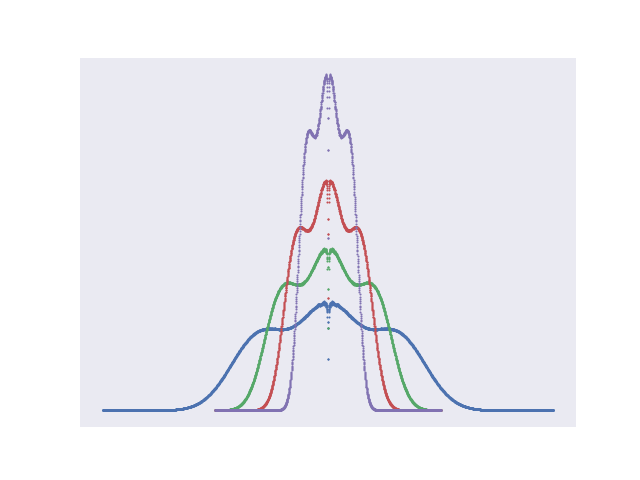
\includegraphics[scale=0.8]{Images/art.png}
	\caption{One-body density plots for 12 particles in a harmonic oscillator well. The four graphs correspond to four different oscillator strengths, where the weakest oscillator gives the broadest density distribution. It's quite artistic, isn't it?}
\end{figure}
After all, this is a Master's degree in physics and the physical results is what is interesting. 
The results are really the heart of this thesis and where most the effort is put... 

We will first highlight some selected results with no repulsive interaction for validation purposes, and then move on to the more realistic case where we look at a larger number of particles for various oscillator strengths and various wave functions structures in two and three dimensions.  

\newpage
\section{Computational cost}
One of the major problems of quantum many-body simulations is the computational cost, which explodes as the system size increases. In figure \eqref{fig:cpu_time} the CPU-time is plotted as a function of full orbitals. 
\begin{figure}[H]
	\centering
	\label{fig:cpu_time}
	\subfloat[2D]{{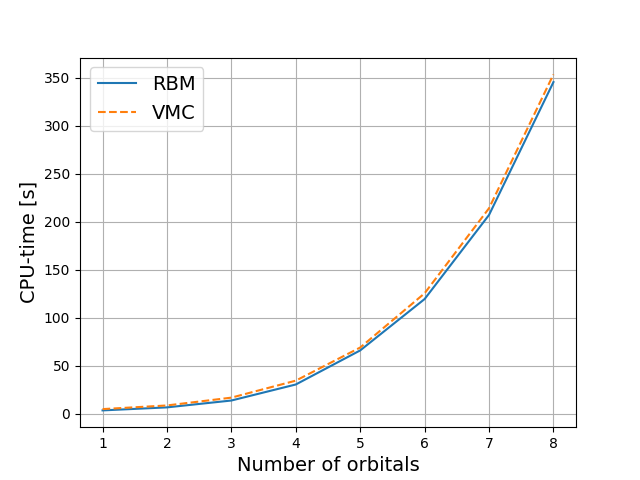
\includegraphics[width=8cm]{/home/evenmn/VMC/plots/cpu_time_2D.png}}}
	\subfloat[3D]{{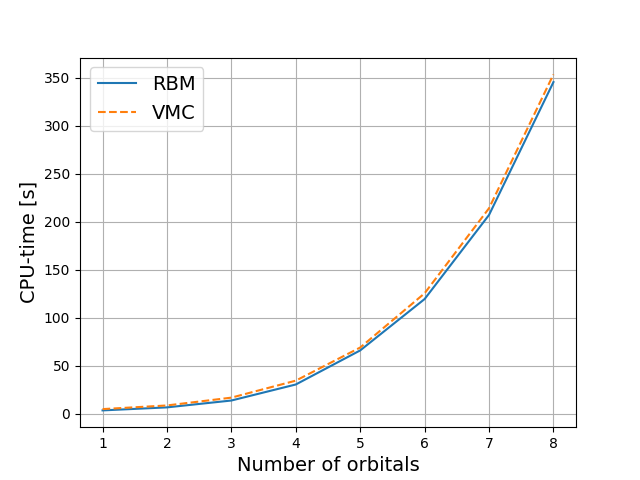
\includegraphics[width=8cm]{/home/evenmn/VMC/plots/cpu_time_2D.png}}}
	\caption{CPU-time as a function of full orbitals for two and three dimensions. The solid line is RBM, while the dashed line is VMC.}
\end{figure}

A quantum many-body simulation is an actual experiment, since the applied theory agrees perfectly with the experiments. In that manner, one can use computer experiments to predict things that is not investigated in real life. Similarly to experiments in a lab, computer experiments are also dependent on external factors, especially when it comes to the CPU-time, and therefore it is important to do such measurements multiple times to find an accurate average time. The CPU-times above are the average from at least four independent runs for each number of orbitals. All the runs were performed on the Abel computational cluster, which is equipped with Supermicro X9DRT compute nodes with dual Intel E5-2670 CPUs running at 2.6 GHz. Different hardware might cause different CPU-times, but the CPU-time ratios (the exponential factor) should be the same. 

For the simulations above, the VMC 2D increases as a power of 3.52

\section{Convergence}
kfkf

\section{No repulsive interaction}
We start with the non-interacting case in order to validate the implemented code. In this case we both know the exact energies and the exact one-body densities for an array of systems, and can therefore test the flexibility of the code. 

\subsection{Ground state energy}
\subsubsection{Quantum dots}
We will start studying systems with no interaction between particles. The number of closed-shell particles are given by equation \eqref{eq:HOclosedshell} and the exact energies are found from formula \eqref{eq:HOenergies}. The first 5 closed-shell energies for $\omega=0.5$ and $\omega=1.0$ are presented in table \eqref{tab:quantumdotswointeraction}.

\begin{table} [H]
	\caption{Energy of $N$ non-interacting electrons trapped in a harmonic oscillator of frequency $\omega=0.5$ and $\omega=1.0$. $E_{\text{RBM}}$ is a single Slater determinant with a plain Boltzmann machine baked in, while $E_{\text{VMC}}$ is standard variational Monte-Carlo.}
	\label{tab:quantumdotswointeraction}
	\begin{tabularx}{\textwidth}{r|r|XXX:XXX} \hline\hline
		\label{tab:nn}
		& $\omega$ & \multicolumn{3}{c}{0.5}&\multicolumn{3}{c}{1.0}\\ \hline
		& $N$ & $E_{\text{RBM}}$ & $E_{\text{VMC}}$ & $E_{\text{exact}}$ & $E_{\text{RBM}}$ & $E_{\text{VMC}}$ & $E_{\text{exact}}$ \\ \hline
		
		\parbox[t]{2mm}{\multirow{5}{*}{\rotatebox[origin=c]{90}{2D}}}
		&2 & 1.00045(5) & 1.0 & 1 & 2.00098(5) & 2.0 & 2\\
		&6 & 5.009(2) & 5.0 & 5 & 10.010(1) & 10.0 & 10 \\
		&12 & - & 14.0 & 14 & - & 28.0 & 28\\
		&20 & - & 30.0 & 30 & - & 60.0 & 60\\
		&30 & - & 55.0 & 55 & - & 110.0 & 110\\ \hline
		
		\parbox[t]{2mm}{\multirow{5}{*}{\rotatebox[origin=c]{90}{3D}}}
		&2 & 1.5050(3) & 1.5 & 1.5 & 3.0063(2) & 3.0 & 3 \\
		&8 & - & 9.0 & 9 & - & 18.0 & 18 \\
		&20 & - & 30.0 & 30 & - & 60.0 & 60 \\
		&40 & - & 75.0 & 75 & - & 150.0 & 150 \\
		&70 & - & 157.5 & 157.5 & - & 315.0 & 315 \\ \hline\hline
	\end{tabularx}
\end{table}
We observe that the NQS wave function is able to reproduce the exact energy for most of the cases, but when the number of particles get large, the statistical error gets significant.

\subsubsection{Atoms}
In the next we will study atoms when the Coulomb interaction is ignored. For those cases, we know the exact answers, given by the Bohr formula presented in equation \eqref{eq:bohrformula}.
\begin{table} [H]
	\caption{The table shows the computed energies of non-interacting atoms with the analytical solution to the right. $E_{\text{RBM}}$ is a single Slater determinant with a plain Boltzmann machine baked in, while $E_{\text{VMC}}$ is standard variational Monte-Carlo.}
	\begin{tabularx}{\textwidth}{X|X|X:X:X} \hline\hline
		\label{tab:nointeractionatoms}
		Atom & $N$ & $E_{\text{RBM}}$ & $E_{\text{VMC}}$ & $E_{\text{exact}}$ \\ \hline
		H & 1 & - & -0.5 & -0.5 \\ 
		He & 2 & - & -4.0 & -4 \\
		Be & 4 & - & - & -20 \\
		Ne & 10 & - & - & -200 \\ \hline\hline
	\end{tabularx}
\end{table}


\subsection{One-body density}
The one-body densities 

\begin{figure} [h]%
	\centering
	\subfloat[2D, $\omega=0.5$]{{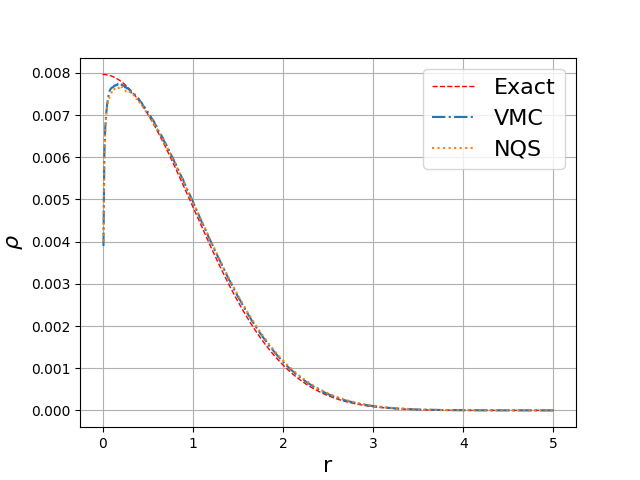
\includegraphics[width=8cm]{/home/evenmn/VMC/plots/int0/onebody/2D/2P/onebody_VMC_NQS_P2_D2_w0p5.png}}}
	\subfloat[2D, $\omega=1.0$]{{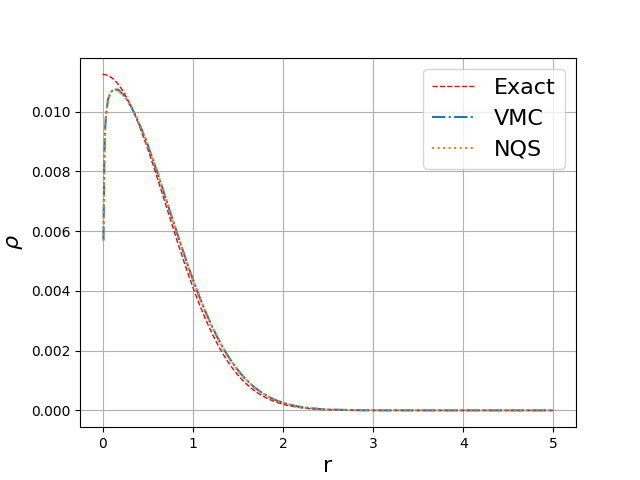
\includegraphics[width=8cm]{/home/evenmn/VMC/plots/int0/onebody/2D/2P/onebody_VMC_NQS_P2_D2_w1p0.png} }}\\
	
	\subfloat[3D, $\omega=0.5$]{{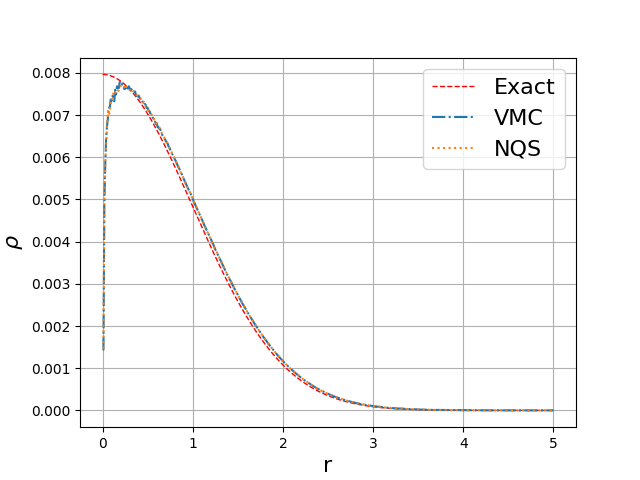
\includegraphics[width=8cm]{/home/evenmn/VMC/plots/int0/onebody/3D/2P/onebody_VMC_NQS_P2_D3_w0p5.png} }}
	\subfloat[3D, $\omega=1.0$]{{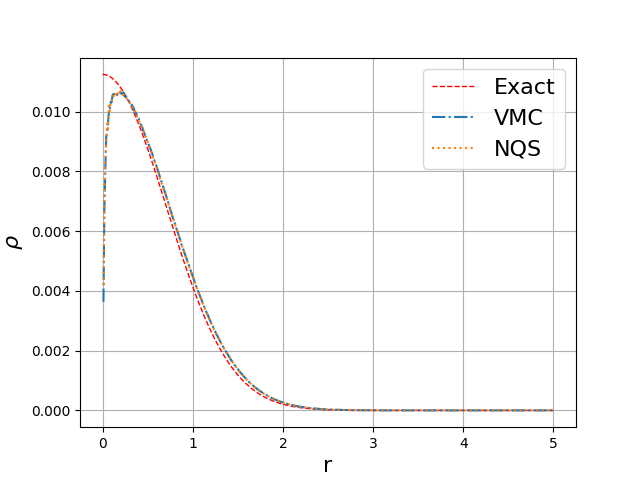
\includegraphics[width=8cm]{/home/evenmn/VMC/plots/int0/onebody/3D/2P/onebody_VMC_NQS_P2_D3_w1p0.png} }}
	\caption{One-body densities of two non-interacting electrons in two dimensions figure (a) and (b) and three dimensions}%
	\label{fig:OB_nointeraction}
\end{figure}

\section{With repulsive interaction}
Now over to the interesting part: the more realistic case with interaction. We no longer have analytical results, apart from a few semi-analytical energies and wave-functions obtained by M. Taut for the two- and three-dimensional harmonic oscillator. More precisely, he found the energy to be $E=3$ for the frequency $\omega=1$ and $E=2/3$ for the frequency $\omega=1/6$ for the two-dimensional case, and $E=2$ for the frequency $\omega=1/2$ and $E=1/2$ for the frequency $\omega=1/10$ for the three-dimensional case. \cite{taut_two_1993}\cite{taut_two_1994}

For other references, we need to rely on what researchers have found before us. Since diffusion Monte-Carlo (DMC) is known to give very accurate results, we will mainly compare our results to J. Høgberget's DMC calculations. \cite{hogberget_quantum_2013} We also run some simulations that we do not have any references for, 

To achieve good results, we applied an adaptive step number, which means that the number of steps per iteration was increased for the last iterations. Firstly, this makes the resulting energies more accurate due to better statistics. Secondly, we get less noisy electron density plots by using this technique. All results below were produced using $2^{20}=1.048.576$ number of steps per iteration for the initial iterations. Then the number of steps was increased to $2^{24}=16.777.216$ when we had 11 iterations left, and for the final iteration we used $2^{28}=268.435.456$ steps. The ADAM optimizer was used.

\begin{landscape}
\subsection{Ground state energy}
\subsubsection{Two dimensions}

\begin{table} [H]
	\caption{This table presents the energies of $N$ electrons trapped in a two-dimensional oscillator well with frequency $\omega$. $E_{\text{RBM}}$ is plain restricted Boltzmann machine (RBM) with Slater determinant, $E_{\text{RBM+PJ}}$ is RBM with Padé-Jastrow factor (PJ), and $E_{\text{VMC}}$ is standard variational Monte-Carlo. The exact energies are calculated analytically by M.Taut, see \cite{taut_two_1994}. The reference is to J. Høgberget's diffusion Monte-Carlo (DMC) calculations \cite{hogberget_quantum_2013}.} 
	\begin{tabularx}{\hsize}{l:l|XXXXXXXX} \hline\hline
		\label{tab:quantumdotswinteraction2D1}
		$N$ & $\omega$ & $E_{\text{RBM+PJ}}$ & $E_{\text{RBM}}$ & $E_{\text{RBM+HF}}$ & $E_{\text{DRBM}}$ & $E_{\text{HF}}$ & $E_{\text{VMC+HF}}$ & $E_{\text{VMC}}$ & $E_{\text{ref}}$ \\ \hline \\
		2 & 0.1 & 0.44130(5) & 0.4731(1) & - & - & - & - & 0.44128(1) & 0.44079(1) \\ 
		& 1/6 & 0.66715(6) & 0.7133(1) & - & - & - & - & 0.66710(1) & $0.6666\bar{6}^{1}$ \\
		& 0.28 & 1.02185(1) & 1.0705(2) & - & - & - & - & 1.02190(1) & 1.02164(1) \\
		& 0.5 & 1.65957(1) & 1.7231(2) & - & - & - & - & 1.65972(1) & 1.65977(1)  \\
		& 1.0 & 3.00002(2) & 3.0822(2) & - & - & - & - & 2.99999(1) & $3.00000^{1}$ \\ \hdashline \\

		6 & 0.1 & 3.5868(6) & 3.719(1) & - & - & - & - & 3.5698(1) & 3.55385(5) \\ 
		& 0.28 & 7.6260(2) & 7.963(8) & - & - & - & - & 7.6219(1) & 7.60019(6) \\
		& 0.5 & 11.8174(2) & 12.265(1) & - & - & - & - & 11.8108(2) & 11.78484(6) \\
		& 1.0 & 20.1893(2) & 20.826(3) & - & - & - & - & 20.1905(2) & 20.15932(8) \\ \hdashline \\
		
		12 & 0.1 & 12.3517(5) & 15.02(6) & - & - & - & - & 12.3201(3) & 12.26984(8) \\ 
		& 0.28 & 25.7645(1) & 26.743(2) & - & - & - & - & 25.7038(4) & 25.63577(9) \\
		& 0.5 & 39.4549(8) & 40.774(3) & - & - & - & - & 39.2660(4) & 39.1596(1) \\
		& 1.0 & 66.047(3) & 67.953(3) & - & - & - & - & 65.7946(8) & 65.7001(1) \\ \hdashline \\
		
		20 & 0.1 & 30.213(1) & 47.4(1) & - & - & - & - & 30.0778(7) & 29.9779(1) \\ 
		& 0.28 & 62.268(3) & 66.578(8) & - & - & - & - & 62.0653(7) & 61.9268(1) \\
		& 0.5 & 94.235(5) & 97.166(5) & - & - & - & - & 94.0391(9) & 93.8752(1) \\
		& 1.0 & 156.205(1) & 160.448(5) & - & - & - & - & 156.106(2) & 155.8822(1) \\ \hdashline
	\end{tabularx}
\end{table}

\begin{table} [H]
	\begin{tabularx}{\hsize}{l:l|XXXXXXXX} \\
		\label{tab:quantumdotswinteraction2D2}
		30 & 0.1 & - & - & - & - & - & - & 60.585(1) & 60.4205(2) \\ 
		& 0.28 & - & 128.00(3) & - & - & - & - & 124.195(2) & 123.9683(2) \\
		& 0.5 & - & 191.683(7) & - & - & - & - & 187.325(3) & 187.0426(2) \\
		& 1.0 & - & 315.26(1) & - & - & - & - & 308.957(2) & 308.5627(2) \\ \hdashline \\
		
		42 & 0.1 & - & - & - & - & - & - & 107.928(2) & 107.6389(2) \\ 
		& 0.28 & - & - & - & - & - & - & 220.224(2) & 219.8426(2) \\
		& 0.5 & - & - & - & - & - & - & 331.276(3) & 330.6306(2) \\
		& 1.0 & - & - & - & - & - & - & 543.738(7) & 542.9428(8) \\ \hdashline \\
		
		56 & 0.1 & - & - & - & - & - & - & 176.774(3) & 175.9553(7) \\ 
		& 0.28 & - & - & - & - & - & - & 359.63(1) & 358.145(2) \\
		& 0.5 & - & - & - & - & - & - & 538.686(9) & 537.353(2) \\
		& 1.0 & - & - & - & - & - & - & 880.352(5) & 879.3986(6) \\ \hdashline \\
		
		72 & 0.1 & - & - & - & - & - & - & 276.83(1) & - \\ 
		& 0.28 & - & - & - & - & - & - & 551.00(2) & - \\
		& 0.5 & - & - & - & - & - & - & 822.82(1) & - \\
		& 1.0 & - & - & - & - & - & - & 1340.520(7) & - \\ \hdashline \\
		
		90 & 0.1 & - & - & - & - & - & - & - & - \\ 
		& 0.28 & - & - & - & - & - & - & - & - \\
		& 0.5 & - & - & - & - & - & - & - & - \\
		& 1.0 & - & - & - & - & - & - & - & - \\ \hline\hline
	\end{tabularx}
\end{table}

\subsubsection{Three dimensions}
\begin{table} [H]
	\caption{This table presents the energies of $N$ electrons trapped in a three-dimensional oscillator well with frequency $\omega$. $E_{\text{RBM}}$ is plain restricted Boltzmann machine (RBM) with Slater determinant, $E_{\text{RBM+PJ}}$ is RBM with Padé-Jastrow factor (PJ), and $E_{\text{VMC}}$ is standard variational Monte-Carlo. The exact energies are calculated analytically by M.Taut, see \cite{taut_two_1993}. The reference is to J. Høgberget's diffusion Monte-Carlo (DMC) calculations \cite{hogberget_quantum_2013}. } 
	\begin{tabularx}{\hsize}{l:l|XXXXXXXX} \hline\hline
		\label{tab:quantumdotswinteraction3D}
		$N$ & $\omega$ & $E_{\text{RBM+PJ}}$ & $E_{\text{RBM}}$ & $E_{\text{RBM+HF}}$ & $E_{\text{DBM}}$ & $E_{\text{HF}}$ & $E_{\text{VMC}}$ & $E_{\text{ref}} $ & $E_{\text{exact}}$ \\ \hline \\
		2 & 0.1 & 0.50073(7) & 0.5253(1) & - & - & - & - & 0.50008(4) & $0.500000^{1}$ \\
		& 0.28 & 1.20201(5) & 1.2284(1) & - & - & - & - & 1.20174(6) & 1.201725(2) \\
		& 0.5 & 2.00009(4) & 2.0270(1) & - & - & - & - & 2.00000(5) & $2.000000^{1}$ \\
		& 1.0 & 3.73032(4) & 3.7571(1) & - & - & - & - & 3.73003(1) & 3.730123(3) \\ \hdashline \\
		
		8 & 0.1 & 5.8448(7) & 6.549(7) & - & - & - & - & 5.8731(9) & 5.7028(1) \\ 
		& 0.28 & 12.2084(2) & 13.098(2) & - & - & - & - & 12.2104(2) & 12.1927(1) \\
		& 0.5 & 18.9831(2) & 19.621(2) & - & - & - & - & 18.9776(2) & 18.9611(1) \\
		& 1.0 & 32.6883(2) & 33.513(1) & - & - & - & - & 32.6846(2) & 32.6680(1) \\ \hdashline \\
		
		20 & 0.1 & - & - & - & - & - & - & 27.72(2) & 27.2717(2) \\ 
		& 0.28 & - & - & - & - & - & - & 56.534(3) & 56.3868(2) \\
		& 0.5 & - & - & - & - & - & - & 85.771(4) & 85.6555(2) \\
		& 1.0 & - & - & - & - & - & - & 142.946(6) & 142.8875(2) \\ \hdashline \\
		
		40 & 0.1 & - & - & - & - & - & - & - & - \\ 
		& 0.28 & - & - & - & - & - & - & - & - \\
		& 0.5 & - & - & - & - & - & - & - & - \\
		& 1.0 & - & - & - & - & - & - & - & - \\ \hdashline \\
		
		70 & 0.1 & - & - & - & - & - & - & 227.082(6) & - \\ 
		& 0.28 & - & - & - & - & - & - & 456.941(2) & - \\
		& 0.5 & - & - & - & - & - & - & 682.277(5) & - \\
		& 1.0 & - & - & - & - & - & - & 1108.950(4) & - \\ \hline\hline
	\end{tabularx}
\end{table}
\end{landscape}

\subsection{One-body densities}
\subsubsection{Two dimensions}
\iffalse
\begin{figure} [H]%
	\centering
	\subfloat[2 particles, RBM]{{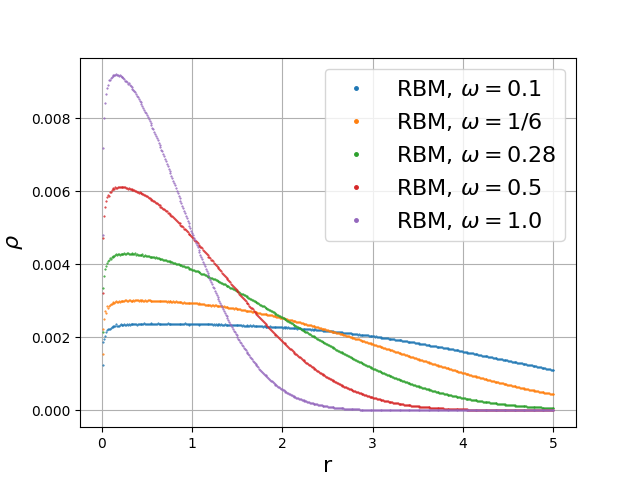
\includegraphics[width=8cm]{/home/evenmn/VMC/doc/plots/int1/onebody/2D/2P/onebody_RBM_2D_2P_SGD.png}}}
	\subfloat[2 particles, VMC]{{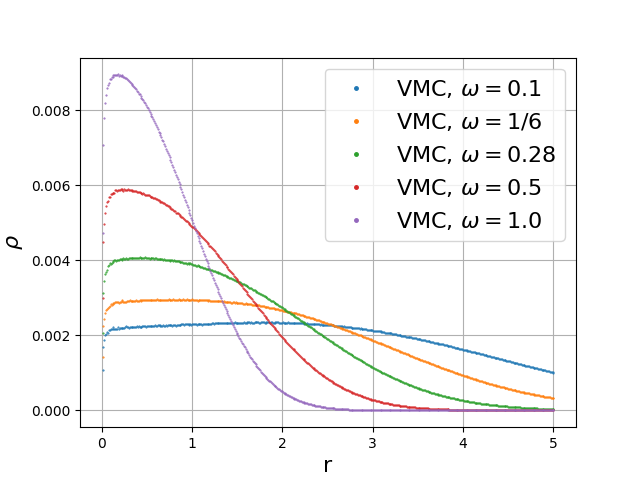
\includegraphics[width=8cm]{/home/evenmn/VMC/doc/plots/int1/onebody/2D/2P/onebody_VMC_2D_2P_SGD.png} }}\\
	
	\subfloat[2 particles RBM \& VMC]{{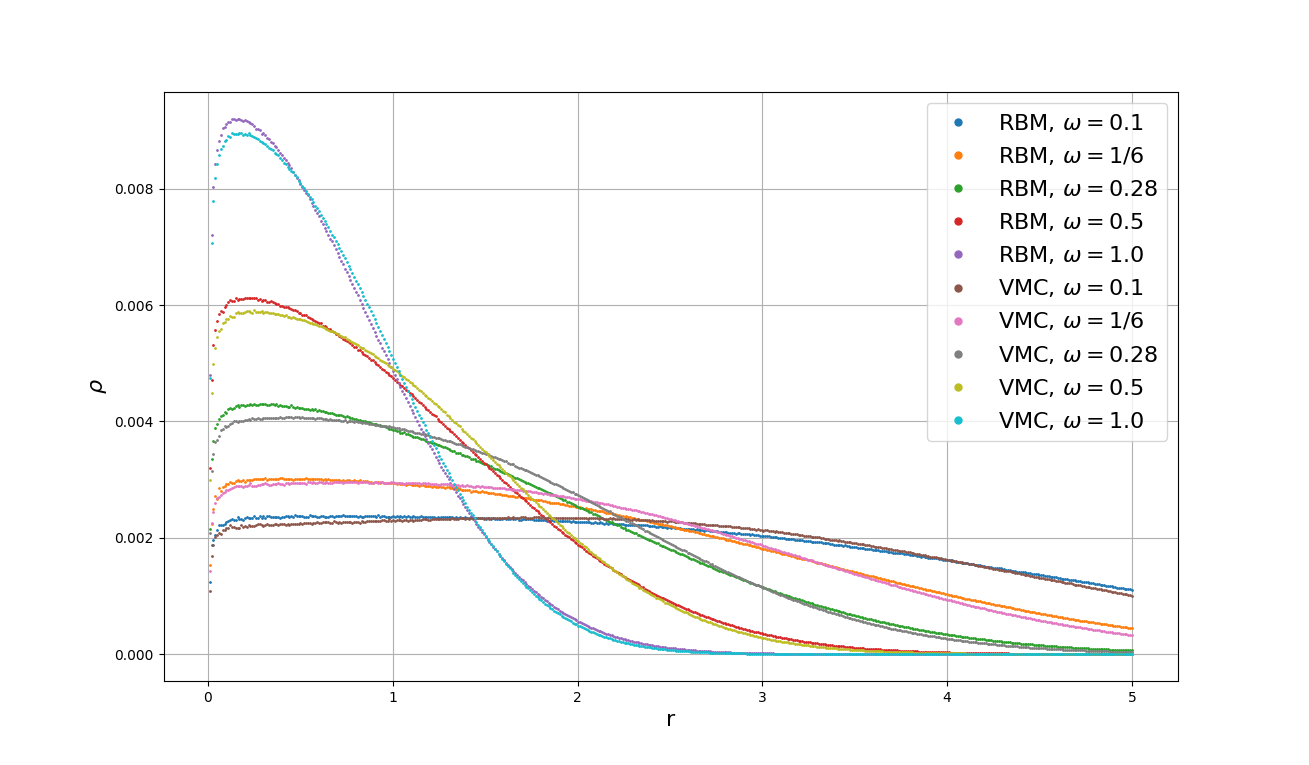
\includegraphics[width=16cm]{/home/evenmn/VMC/doc/plots/int1/onebody/2D/2P/onebody_VMC_RBM_2D_2P_SGD.png} }}
	%\subfloat[20 particles]{{
\includegraphics[width=6cm]{Images/example.png} }}
	\caption{One-body densities of two non-interacting electrons in two dimensions for various oscillator frequencies produced by standard variational Monte-Carlo (VMC) and plain restricted Boltzmann machine (RBM). Stochastic gradient descent was used, and after convergence the number of Monte-Carlo cycles was $MC=2^{28}=268.435.456$}%
	\label{fig:OB_interaction_2P_2D2}
\end{figure}
\fi

\begin{figure} [H]%
	\centering
	\subfloat[$\omega=0.1$]{{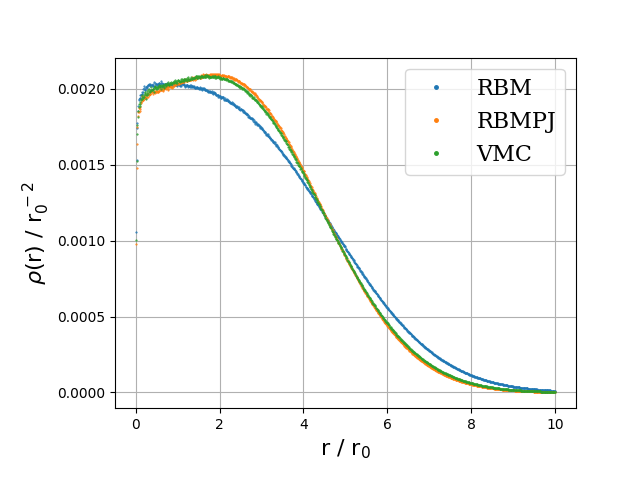
\includegraphics[width=8cm]{/home/evenmn/VMC/plots/int1/onebody/2D/2P/0.100000w/2D_2P_0p100000w_MC2pow28.png}}}
	\subfloat[$\omega=0.28$]{{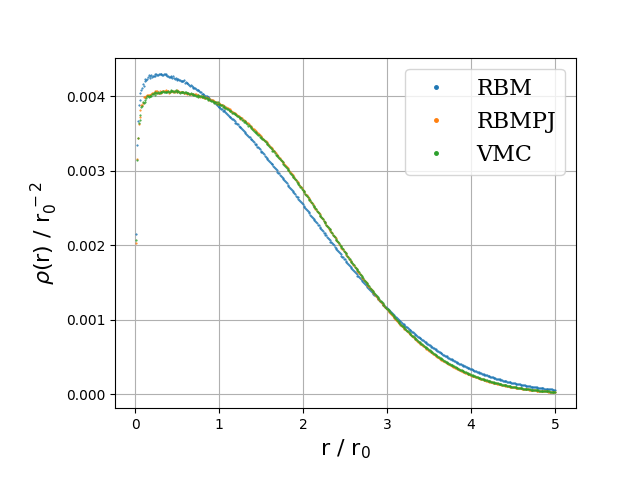
\includegraphics[width=8cm]{/home/evenmn/VMC/plots/int1/onebody/2D/2P/0.280000w/2D_2P_0p280000w_MC2pow28.png}}}\\
	
	\subfloat[$\omega=0.5$]{{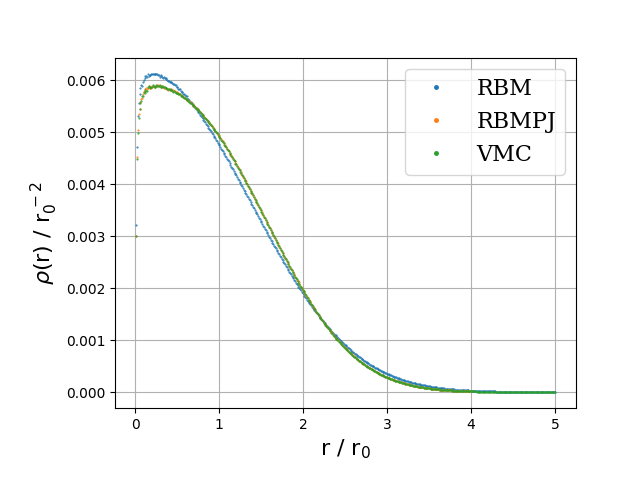
\includegraphics[width=8cm]{/home/evenmn/VMC/plots/int1/onebody/2D/2P/0.500000w/2D_2P_0p500000w_MC2pow28.png}}}
	\subfloat[$\omega=1.0$]{{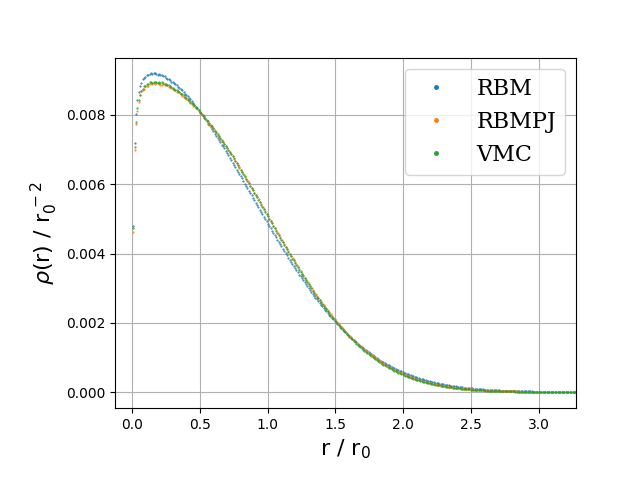
\includegraphics[width=8cm]{/home/evenmn/VMC/plots/int1/onebody/2D/2P/1.000000w/2D_2P_1p000000w_MC2pow28.png}}}
	\caption{One-body densities of two interacting electrons in two dimensions for various oscillator frequencies produced by standard variational Monte-Carlo (VMC), plain restricted Boltzmann machine (RBM) and restricted Boltzmann machine with Padé-Jastrow factor (RBMPJ). Stochastic gradient descent was used, and after convergence the number of Monte-Carlo cycles was $MC=2^{28}=268.435.456$.}%
	\label{fig:OB_interaction_2P_2D}
\end{figure}

\iffalse
\begin{figure} [H]%
	\centering
	\subfloat[6 particles, RBM]{{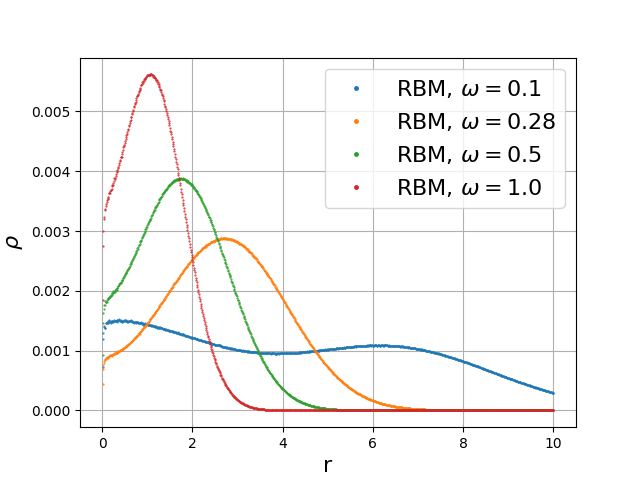
\includegraphics[width=8cm]{/home/evenmn/VMC/doc/plots/int1/onebody/2D/6P/onebody_RBM_2D_6P_SGD.png}}}
	\subfloat[6 particles, VMC]{{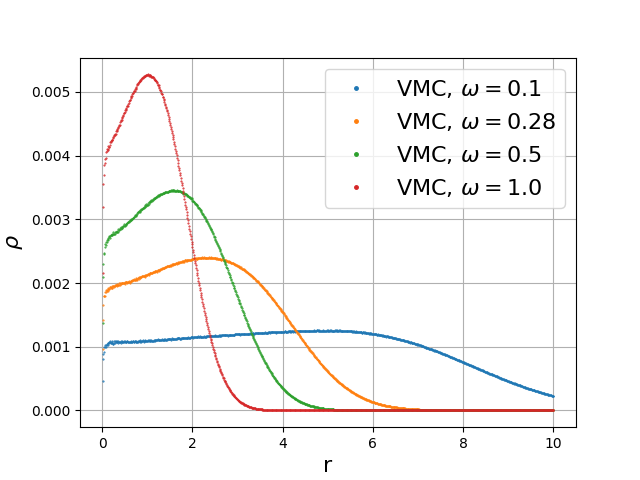
\includegraphics[width=8cm]{/home/evenmn/VMC/doc/plots/int1/onebody/2D/6P/onebody_VMC_2D_6P_SGD.png} }}\\
	
	\subfloat[6 particles RBM \& VMC]{{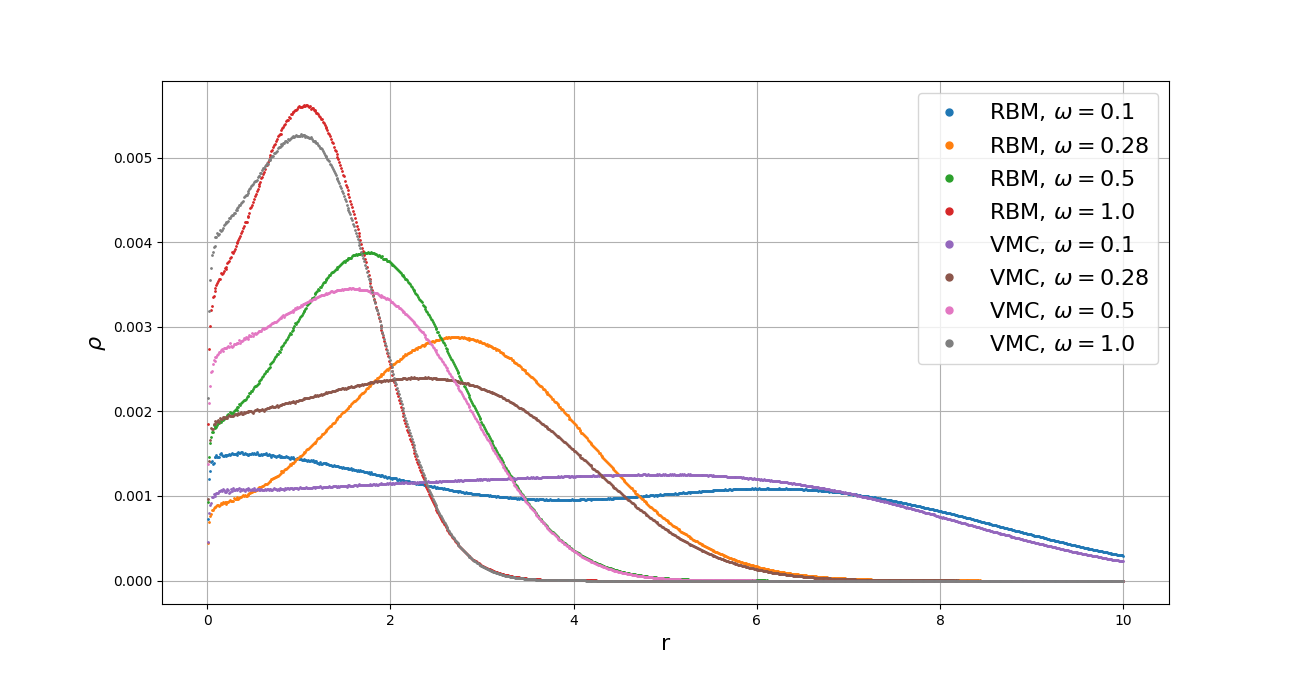
\includegraphics[width=16cm]{/home/evenmn/VMC/doc/plots/int1/onebody/2D/6P/onebody_VMC_RBM_2D_6P_SGD.png} }}
	%\subfloat[20 particles]{{
\includegraphics[width=6cm]{Images/example.png} }}
	\caption{One-body densities of six interacting electrons in two dimensions for various oscillator frequencies produced by standard variational Monte-Carlo (VMC) and plain restricted Boltzmann machine (RBM). Stochastic gradient descent was used, and after convergence the number of Monte-Carlo cycles was $MC=2^{28}=268.435.456$}%
	\label{fig:OB_interaction_6P_2D2}
\end{figure}
\fi

\begin{figure} [H]%
	\centering
	\subfloat[$\omega=0.1$]{{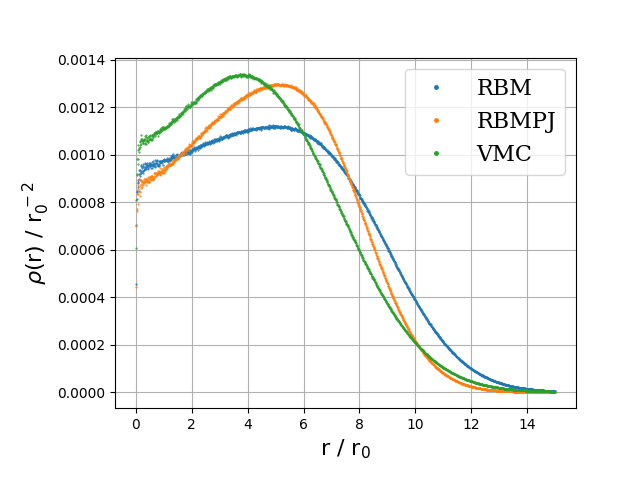
\includegraphics[width=8cm]{/home/evenmn/VMC/plots/int1/onebody/2D/6P/0.100000w/2D_6P_0p100000w_MC2pow28.png}}}
	\subfloat[$\omega=0.28$]{{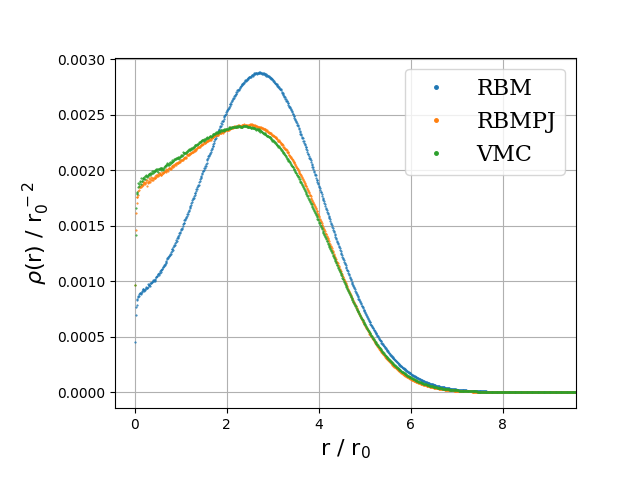
\includegraphics[width=8cm]{/home/evenmn/VMC/plots/int1/onebody/2D/6P/0.280000w/2D_6P_0p280000w_MC2pow28.png}}}\\
	
	\subfloat[$\omega=0.5$]{{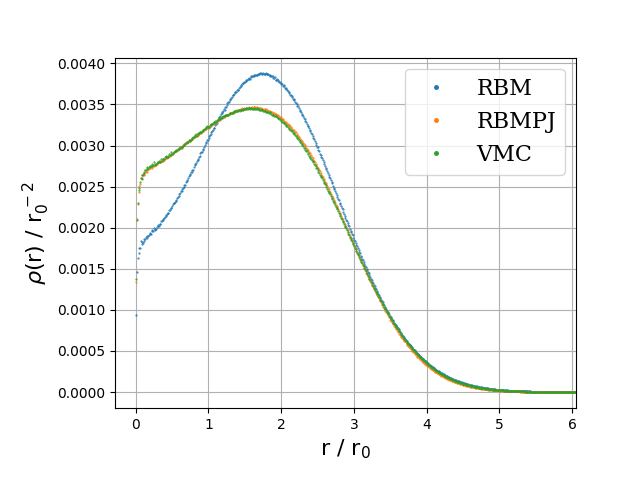
\includegraphics[width=8cm]{/home/evenmn/VMC/plots/int1/onebody/2D/6P/0.500000w/2D_6P_0p500000w_MC2pow28.png}}}
	\subfloat[$\omega=1.0$]{{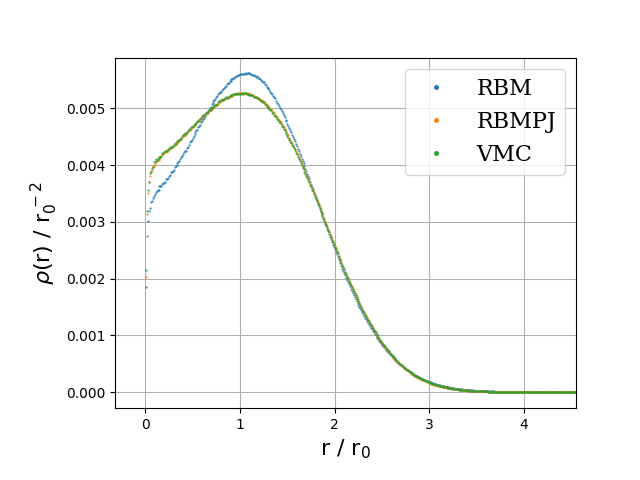
\includegraphics[width=8cm]{/home/evenmn/VMC/plots/int1/onebody/2D/6P/1.000000w/2D_6P_1p000000w_MC2pow28.png}}}
	\caption{One-body densities of six interacting electrons in two dimensions for various oscillator frequencies produced by standard variational Monte-Carlo (VMC), plain restricted Boltzmann machine (RBM) and restricted Boltzmann machine with Padé-Jastrow factor (RBMPJ). Stochastic gradient descent was used, and after convergence the number of Monte-Carlo cycles was $MC=2^{28}=268.435.456$.}%
	\label{fig:OB_interaction_6P_2D}
\end{figure}

\iffalse
\begin{figure} [H]%
	\centering
	\subfloat[12 particles, RBM]{{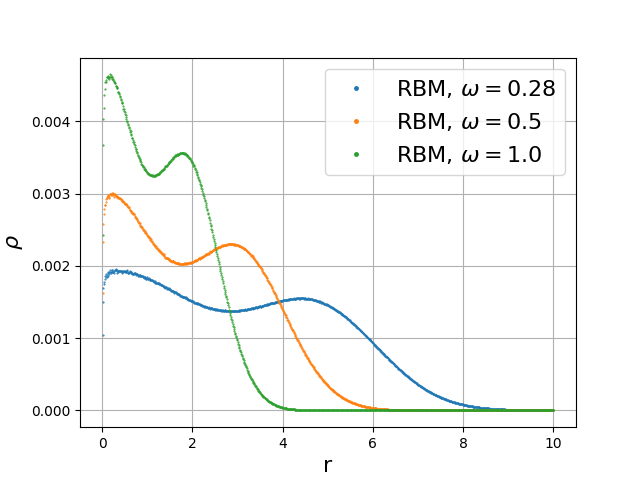
\includegraphics[width=8cm]{/home/evenmn/VMC/doc/plots/int1/onebody/2D/12P/onebody_RBM_2D_12P_SGD.png}}}
	\subfloat[12 particles, VMC]{{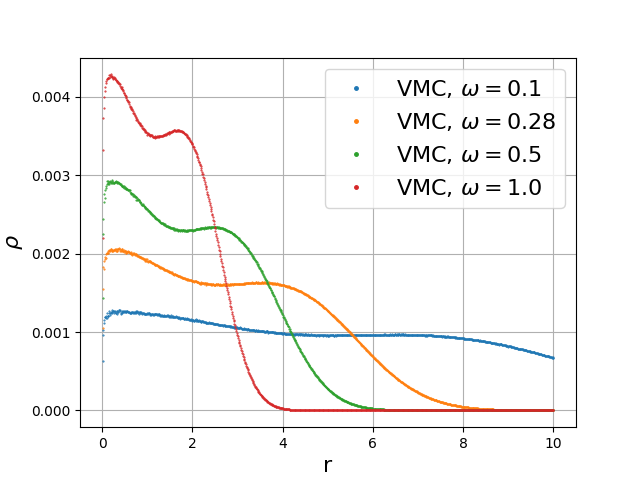
\includegraphics[width=8cm]{/home/evenmn/VMC/doc/plots/int1/onebody/2D/12P/onebody_VMC_2D_12P_SGD.png} }}\\
	
	\subfloat[12 particles RBM \& VMC]{{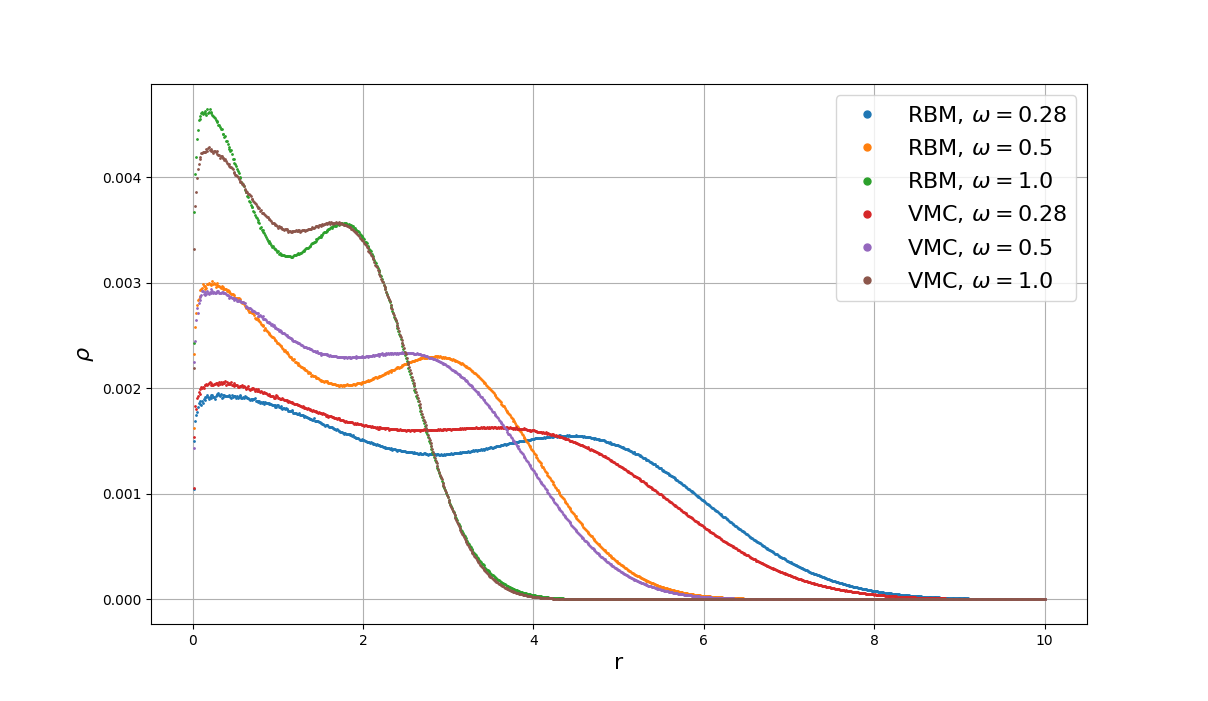
\includegraphics[width=16cm]{/home/evenmn/VMC/doc/plots/int1/onebody/2D/12P/onebody_VMC_RBM_2D_12P_SGD.png} }}
	%\subfloat[20 particles]{{
\includegraphics[width=6cm]{Images/example.png} }}
	\caption{One-body densities of 12 interacting electrons in two dimensions for various oscillator frequencies produced by standard variational Monte-Carlo (VMC) and plain restricted Boltzmann machine (RBM). Stochastic gradient descent was used, and after convergence the number of Monte-Carlo cycles was $MC=2^{28}=268.435.456$}%
	\label{fig:OB_interaction_12P_2D2}
\end{figure}
\fi

\begin{figure} [H]%
	\centering
	\subfloat[$\omega=0.1$]{{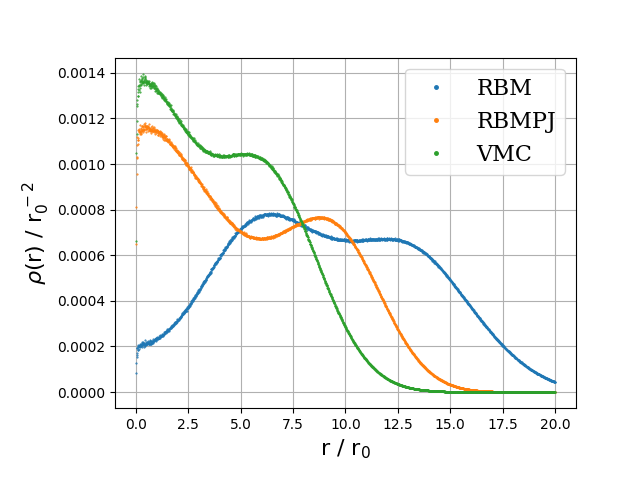
\includegraphics[width=8cm]{/home/evenmn/VMC/plots/int1/onebody/2D/12P/0.100000w/2D_12P_0p100000w_MC2pow28.png}}}
	\subfloat[$\omega=0.28$]{{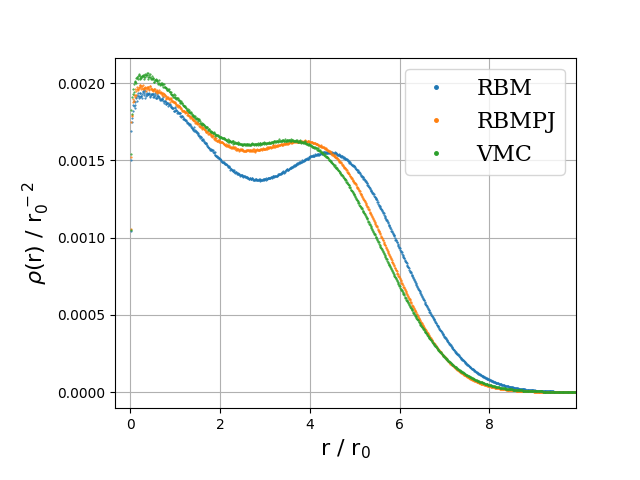
\includegraphics[width=8cm]{/home/evenmn/VMC/plots/int1/onebody/2D/12P/0.280000w/2D_12P_0p280000w_MC2pow28.png}}}\\
	
	\subfloat[$\omega=0.5$]{{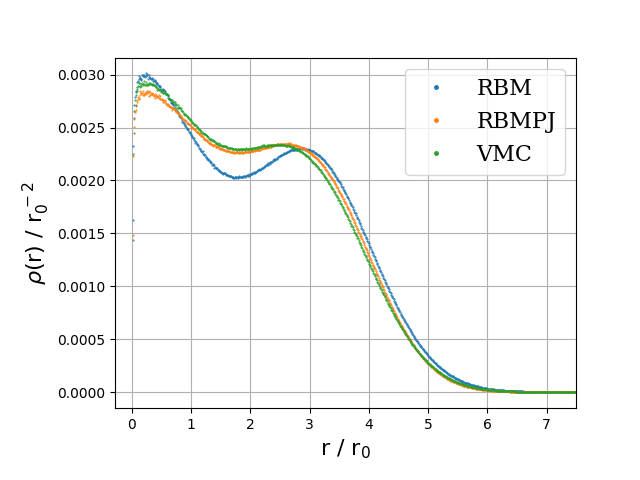
\includegraphics[width=8cm]{/home/evenmn/VMC/plots/int1/onebody/2D/12P/0.500000w/2D_12P_0p500000w_MC2pow28.png}}}
	\subfloat[$\omega=1.0$]{{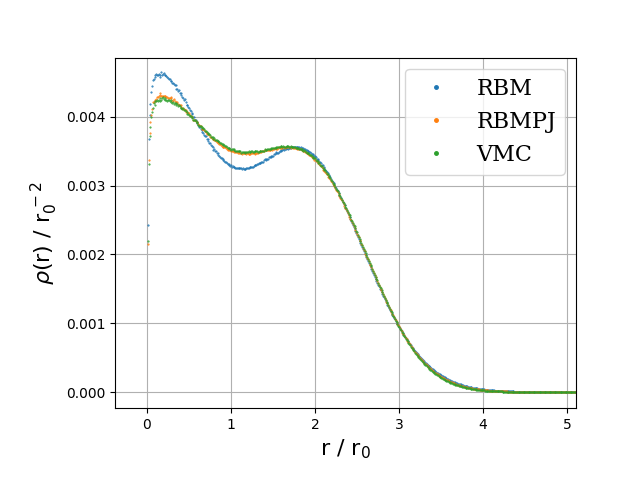
\includegraphics[width=8cm]{/home/evenmn/VMC/plots/int1/onebody/2D/12P/1.000000w/2D_12P_1p000000w_MC2pow28.png}}}
	\caption{One-body densities of 12 interacting electrons in two dimensions for various oscillator frequencies produced by standard variational Monte-Carlo (VMC), plain restricted Boltzmann machine (RBM) and restricted Boltzmann machine with Padé-Jastrow factor (RBMPJ). Stochastic gradient descent was used, and after convergence the number of Monte-Carlo cycles was $MC=2^{28}=268.435.456$.}%
	\label{fig:OB_interaction_12P_2D}
\end{figure}

\begin{figure} [H]%
	\centering
	\subfloat[$\omega=0.1$]{{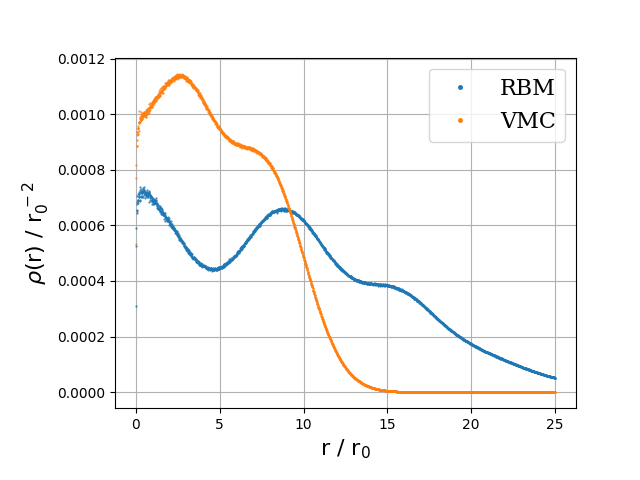
\includegraphics[width=8cm]{/home/evenmn/VMC/plots/int1/onebody/2D/20P/0.100000w/2D_20P_0p100000w_MC2pow28.png}}}
	\subfloat[$\omega=0.28$]{{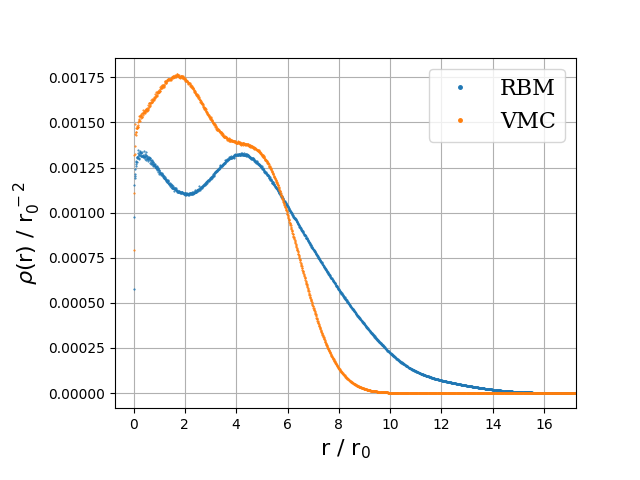
\includegraphics[width=8cm]{/home/evenmn/VMC/plots/int1/onebody/2D/20P/0.280000w/2D_20P_0p280000w_MC2pow28.png}}}\\
	
	\subfloat[$\omega=0.5$]{{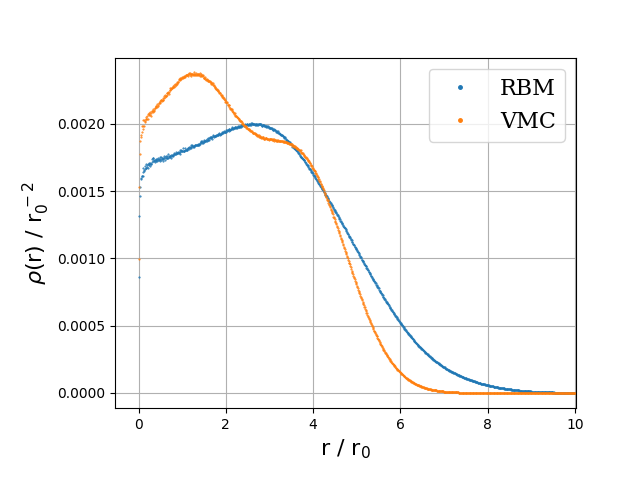
\includegraphics[width=8cm]{/home/evenmn/VMC/plots/int1/onebody/2D/20P/0.500000w/2D_20P_0p500000w_MC2pow28.png}}}
	\subfloat[$\omega=1.0$]{{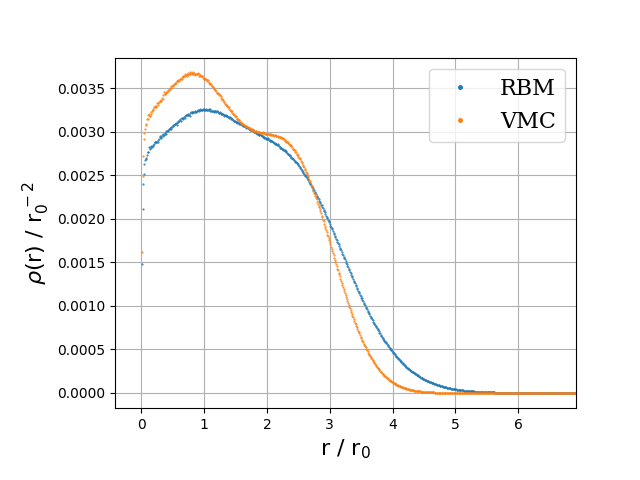
\includegraphics[width=8cm]{/home/evenmn/VMC/plots/int1/onebody/2D/20P/1.000000w/2D_20P_1p000000w_MC2pow28.png}}}
	\caption{One-body densities of 20 interacting electrons in two dimensions for various oscillator frequencies produced by standard variational Monte-Carlo (VMC), plain restricted Boltzmann machine (RBM) and restricted Boltzmann machine with Padé-Jastrow factor (RBMPJ). Stochastic gradient descent was used, and after convergence the number of Monte-Carlo cycles was $MC=2^{28}=268.435.456$.}%
	\label{fig:OB_interaction_20P_2D}
\end{figure}

\begin{figure} [H]%
	\centering
	\subfloat[$\omega=0.1$]{{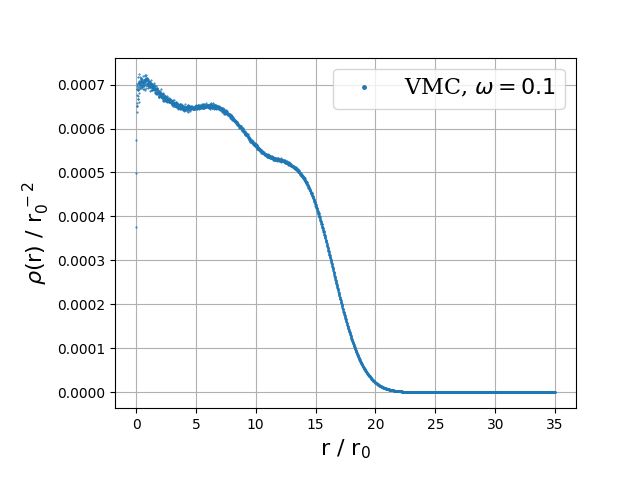
\includegraphics[width=8cm]{/home/evenmn/VMC/plots/int1/onebody/2D/30P/0.100000w/2D_30P_0p100000w_MC2pow28.png}}}
	\subfloat[$\omega=0.28$]{{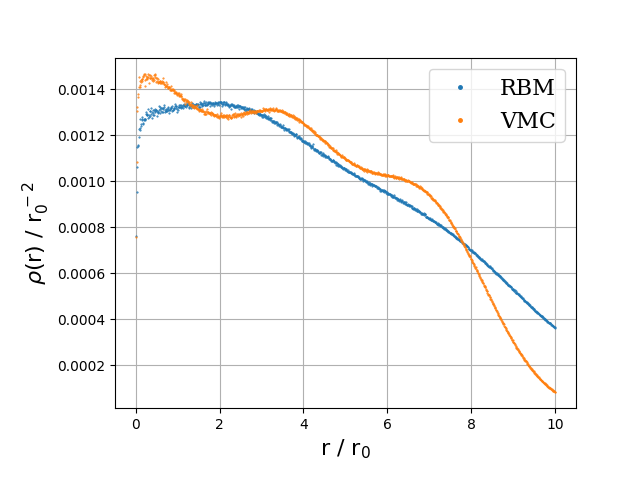
\includegraphics[width=8cm]{/home/evenmn/VMC/plots/int1/onebody/2D/30P/0.280000w/2D_30P_0p280000w_MC2pow28.png}}}\\
	
	\subfloat[$\omega=0.5$]{{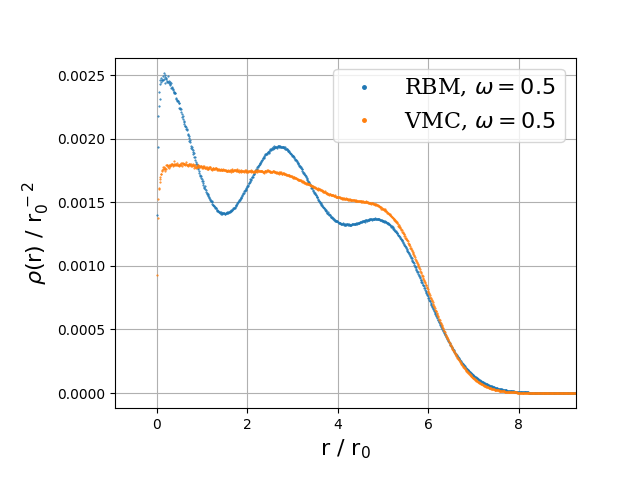
\includegraphics[width=8cm]{/home/evenmn/VMC/plots/int1/onebody/2D/30P/0.500000w/2D_30P_0p500000w_MC2pow28.png}}}
	\subfloat[$\omega=1.0$]{{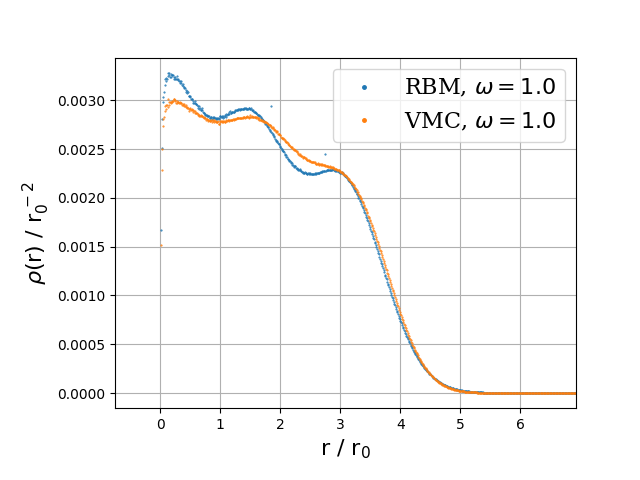
\includegraphics[width=8cm]{/home/evenmn/VMC/plots/int1/onebody/2D/30P/1.000000w/2D_30P_1p000000w_MC2pow28.png}}}
	\caption{One-body densities of 30 interacting electrons in two dimensions for various oscillator frequencies produced by standard variational Monte-Carlo (VMC), plain restricted Boltzmann machine (RBM) and restricted Boltzmann machine with Padé-Jastrow factor (RBMPJ). Stochastic gradient descent was used, and after convergence the number of Monte-Carlo cycles was $MC=2^{28}=268.435.456$.}%
	\label{fig:OB_interaction_30P_2D}
\end{figure}

\subsubsection{Three dimensions}
\iffalse
\begin{figure} [H]%
	\centering
	\subfloat[2 particles, RBM]{{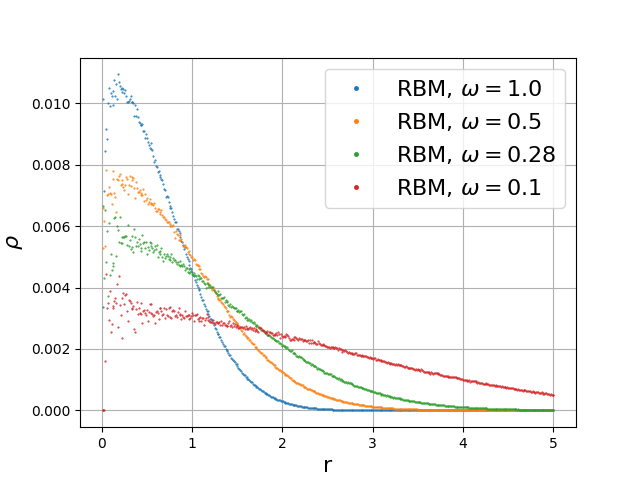
\includegraphics[width=8cm]{/home/evenmn/VMC/plots/int1/onebody/3D/2P/onebody_NQS_P2_D3_allfreq.png}}}
	\subfloat[2 particles, VMC]{{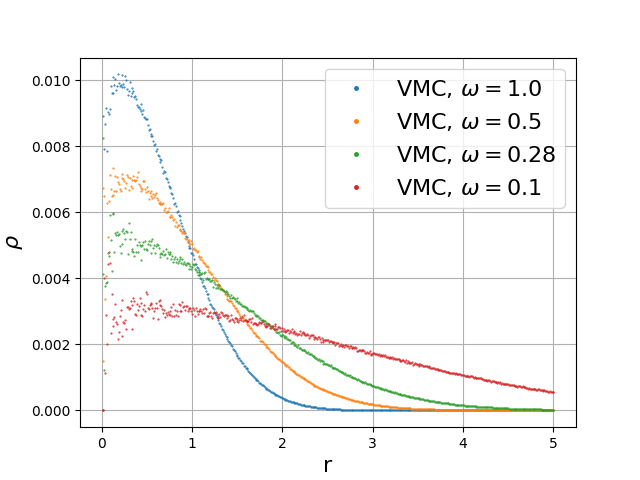
\includegraphics[width=8cm]{/home/evenmn/VMC/plots/int1/onebody/3D/2P/onebody_VMC_P2_D3_allfreq.png} }}\\
	
	\subfloat[2 particles RBM \& VMC]{{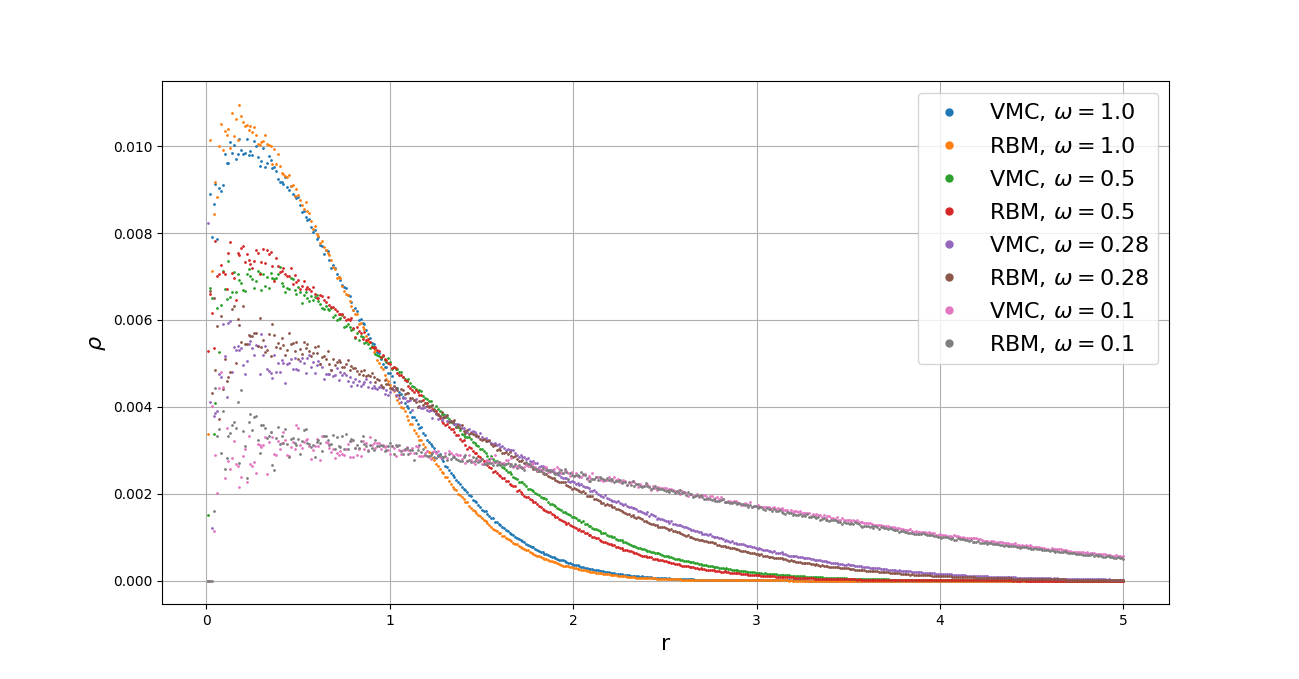
\includegraphics[width=16cm]{/home/evenmn/VMC/plots/int1/onebody/3D/2P/onebody_VMC_NQS_P2_D3_allfreq.png} }}
	%\subfloat[20 particles]{{
\includegraphics[width=6cm]{Images/example.png} }}
	\caption{One-body densities of two interacting electrons in three dimensions for various oscillator frequencies produced by standard variational Monte-Carlo (VMC) and plain restricted Boltzmann machine (RBM). Stochastic gradient descent was used, and after convergence the number of Monte-Carlo cycles was $MC=2^{28}=268.435.456$}%
	\label{fig:OB_interaction_2P_3D2}
\end{figure}
\fi

\begin{figure} [H]%
	\centering
		\subfloat[$\omega=0.1$]{{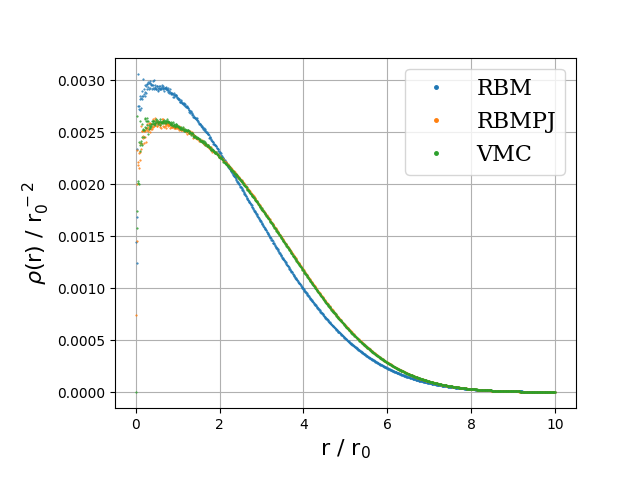
\includegraphics[width=8cm]{/home/evenmn/VMC/plots/int1/onebody/3D/2P/0.100000w/3D_2P_0p100000w_MC2pow28.png}}}
	\subfloat[$\omega=0.28$]{{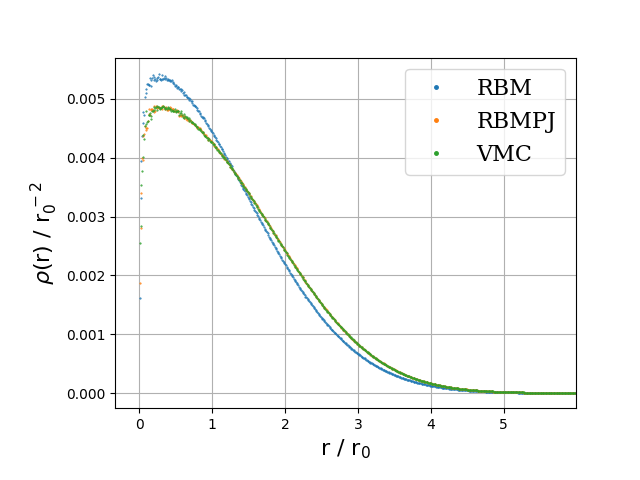
\includegraphics[width=8cm]{/home/evenmn/VMC/plots/int1/onebody/3D/2P/0.280000w/3D_2P_0p280000w_MC2pow28.png}}}\\
	
	\subfloat[$\omega=0.5$]{{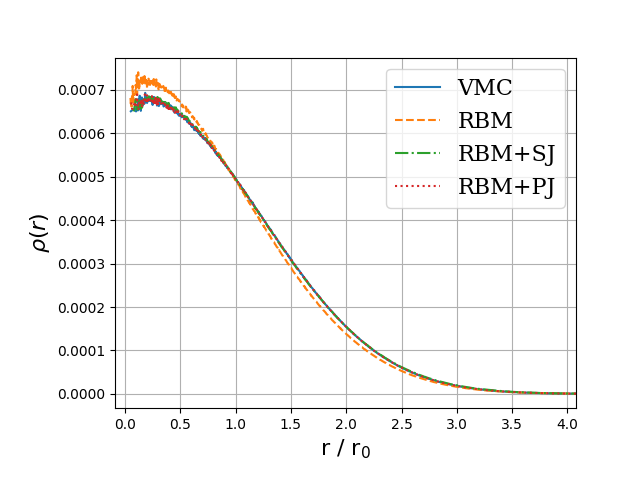
\includegraphics[width=8cm]{/home/evenmn/VMC/plots/int1/onebody/3D/2P/0.500000w/3D_2P_0p500000w_MC2pow28.png}}}
	\subfloat[$\omega=1.0$]{{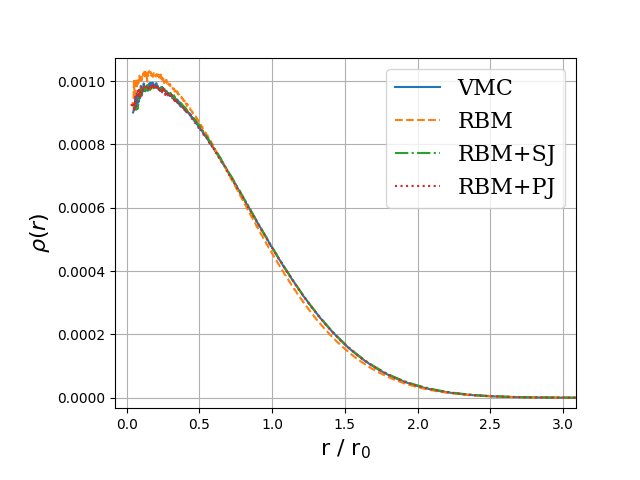
\includegraphics[width=8cm]{/home/evenmn/VMC/plots/int1/onebody/3D/2P/1.000000w/3D_2P_1p000000w_MC2pow28.png}}}
	\caption{One-body densities of two interacting electrons in three dimensions for various oscillator frequencies produced by standard variational Monte-Carlo (VMC), plain restricted Boltzmann machine (RBM) and restricted Boltzmann machine with Padé-Jastrow factor (RBMPJ). Stochastic gradient descent was used, and after convergence the number of Monte-Carlo cycles was $MC=2^{28}=268.435.456$.}%
	\label{fig:OB_interaction_2P_3D}
\end{figure}

\iffalse
\begin{figure} [H]%
	\centering
	\subfloat[8 particles, RBM]{{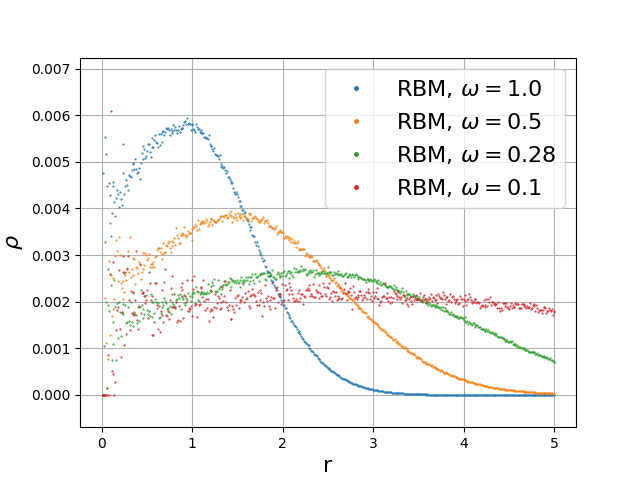
\includegraphics[width=8cm]{/home/evenmn/VMC/plots/int1/onebody/3D/8P/onebody_NQS_P8_D3_allfreq.png}}}
	\subfloat[8 particles, VMC]{{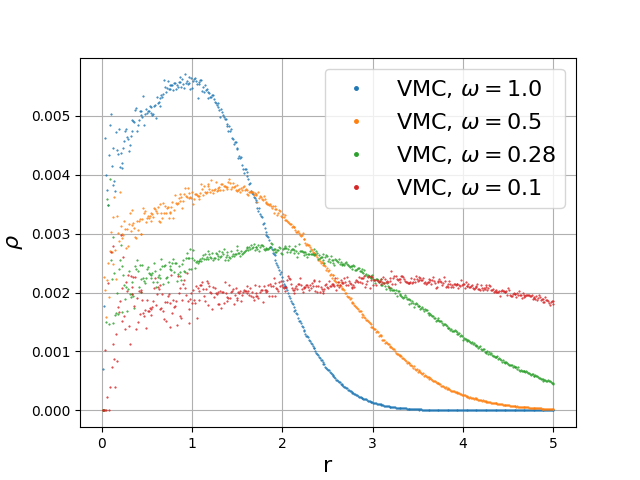
\includegraphics[width=8cm]{/home/evenmn/VMC/plots/int1/onebody/3D/8P/onebody_VMC_P8_D3_allfreq.png} }}\\
	
	\subfloat[8 particles RBM \& VMC]{{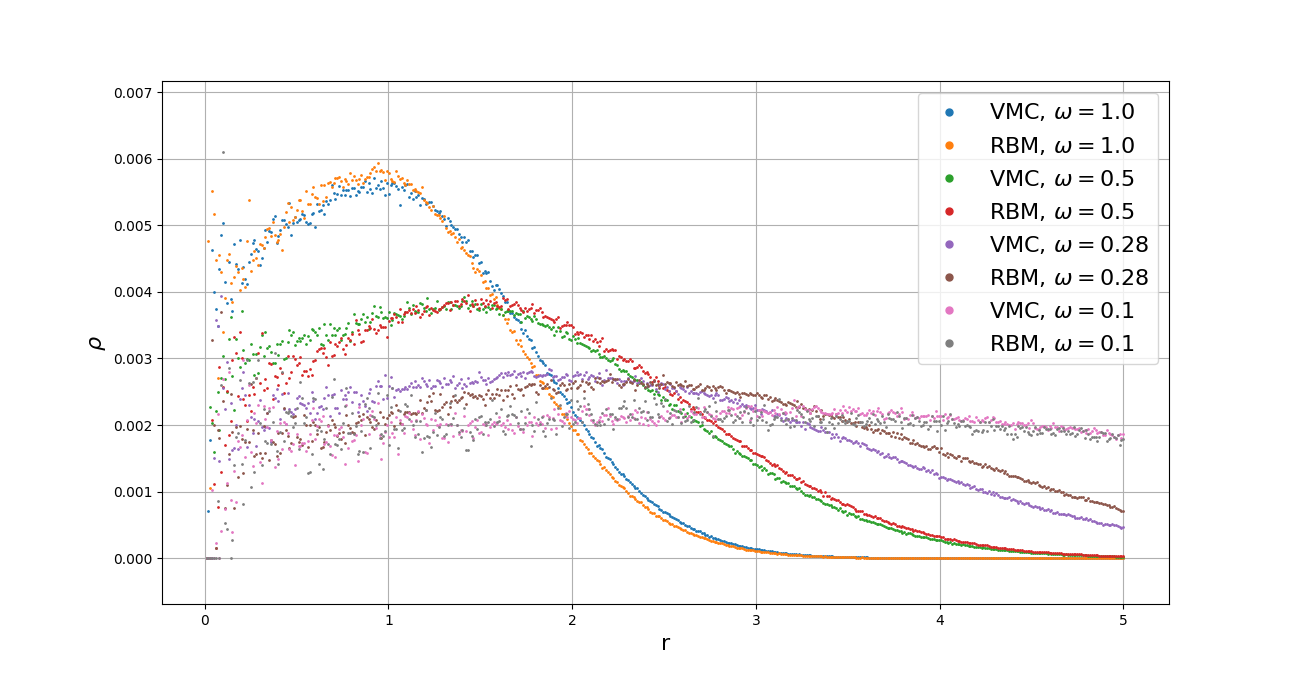
\includegraphics[width=16cm]{/home/evenmn/VMC/plots/int1/onebody/3D/8P/onebody_VMC_NQS_P8_D3_allfreq.png} }}
	%\subfloat[20 particles]{{\includegraphics[width=6cm]{Images/example.png} }}
	\caption{One-body densities of eight non-interacting electrons in three dimensions for various oscillator frequencies produced by standard variational Monte-Carlo (VMC) and plain restricted Boltzmann machine (RBM). Stochastic gradient descent was used, and after convergence the number of Monte-Carlo cycles was $MC=2^{28}=268.435.456$}%
	\label{fig:OB_interaction_8P_3D2}
\end{figure}
\fi

\begin{figure} [H]%
	\centering
	\subfloat[$\omega=0.1$]{{\includegraphics[width=8cm]{/home/evenmn/VMC/plots/int1/onebody/3D/8P/0.100000w/3D_8P_0p100000w_MC2pow28.png}}}
	\subfloat[$\omega=0.28$]{{\includegraphics[width=8cm]{/home/evenmn/VMC/plots/int1/onebody/3D/8P/0.280000w/3D_8P_0p280000w_MC2pow28.png}}}\\
	
	\subfloat[$\omega=0.5$]{{\includegraphics[width=8cm]{/home/evenmn/VMC/plots/int1/onebody/3D/8P/0.500000w/3D_8P_0p500000w_MC2pow28.png}}}
	\subfloat[$\omega=1.0$]{{\includegraphics[width=8cm]{/home/evenmn/VMC/plots/int1/onebody/3D/8P/1.000000w/3D_8P_1p000000w_MC2pow28.png}}}
	\caption{One-body densities for eight interacting electrons in three dimensions for various oscillator frequencies produced by standard variational Monte-Carlo (VMC) and plain restricted Boltzmann machine (RBM). Stochastic gradient descent was used, and after convergence the number of Monte-Carlo cycles was $MC=2^{28}=268.435.456$}%
	\label{fig:OB_interaction_8P_3D}
\end{figure}

\begin{figure} [H]%
	\centering
	\subfloat[$\omega=0.1$]{{\includegraphics[width=8cm]{/home/evenmn/VMC/plots/int1/onebody/3D/8P/0.100000w/3D_8P_0p100000w_MC2pow28.png}}}
	\subfloat[$\omega=0.28$]{{\includegraphics[width=8cm]{/home/evenmn/VMC/plots/int1/onebody/3D/8P/0.280000w/3D_8P_0p280000w_MC2pow28.png}}}\\
	
	\subfloat[$\omega=0.5$]{{\includegraphics[width=8cm]{/home/evenmn/VMC/plots/int1/onebody/3D/8P/0.500000w/3D_8P_0p500000w_MC2pow28.png}}}
	\subfloat[$\omega=1.0$]{{\includegraphics[width=8cm]{/home/evenmn/VMC/plots/int1/onebody/3D/8P/1.000000w/3D_8P_1p000000w_MC2pow28.png}}}
	\caption{One-body densities of eight interacting electrons in three dimensions for various oscillator frequencies produced by standard variational Monte-Carlo (VMC), plain restricted Boltzmann machine (RBM) and restricted Boltzmann machine with Padé-Jastrow factor (RBMPJ). Stochastic gradient descent was used, and after convergence the number of Monte-Carlo cycles was $MC=2^{28}=268.435.456$.}%
	\label{fig:OB_interaction_12P_3D}
\end{figure}

\subsection{Two-body density plots}
\subsubsection{Two dimensions}
\begin{figure} [H]%
	\centering
	\subfloat[RBM+PJ, $\omega=0.1$]{{\includegraphics[width=6cm]{/home/evenmn/VMC/plots/int1/twobody/2D/2P/0.100000w/RBM_2D_2P_0p100000w_MC2pow28.png}}}
	\subfloat[RBM, $\omega=0.1$]{{\includegraphics[width=6cm]{/home/evenmn/VMC/plots/int1/twobody/2D/2P/0.100000w/RBM_2D_2P_0p100000w_MC2pow28.png}}}
	\subfloat[VMC, $\omega=0.1$]{{\includegraphics[width=6cm]{/home/evenmn/VMC/plots/int1/twobody/2D/2P/0.100000w/VMC_2D_2P_0p100000w_MC2pow28.png}}}\\
	
	\subfloat[RBM+PJ, $\omega=0.28$]{{\includegraphics[width=6cm]{/home/evenmn/VMC/plots/int1/twobody/2D/2P/0.280000w/VMC_2D_2P_0p280000w_MC2pow28.png}}}
	\subfloat[RBM, $\omega=0.28$]{{\includegraphics[width=6cm]{/home/evenmn/VMC/plots/int1/twobody/2D/2P/0.280000w/VMC_2D_2P_0p280000w_MC2pow28.png}}}
	\subfloat[VMC, $\omega=0.28$]{{\includegraphics[width=6cm]{/home/evenmn/VMC/plots/int1/twobody/2D/2P/0.280000w/VMC_2D_2P_0p280000w_MC2pow28.png}}}\\
	
	\subfloat[RBM+PJ, $\omega=0.5$]{{\includegraphics[width=6cm]{/home/evenmn/VMC/plots/int1/twobody/2D/2P/0.500000w/RBM_2D_2P_0p500000w_MC2pow28.png}}}
	\subfloat[RBM, $\omega=0.5$]{{\includegraphics[width=6cm]{/home/evenmn/VMC/plots/int1/twobody/2D/2P/0.500000w/RBM_2D_2P_0p500000w_MC2pow28.png}}}
	\subfloat[VMC, $\omega=0.5$]{{\includegraphics[width=6cm]{/home/evenmn/VMC/plots/int1/twobody/2D/2P/0.500000w/VMC_2D_2P_0p500000w_MC2pow28.png}}}\\
	
	\subfloat[RBM+PJ, $\omega=1.0$]{{\includegraphics[width=6cm]{/home/evenmn/VMC/plots/int1/twobody/2D/2P/1.000000w/RBM_2D_2P_1p000000w_MC2pow28.png}}}
	\subfloat[RBM, $\omega=1.0$]{{\includegraphics[width=6cm]{/home/evenmn/VMC/plots/int1/twobody/2D/2P/1.000000w/RBM_2D_2P_1p000000w_MC2pow28.png}}}
	\subfloat[VMC, $\omega=1.0$]{{\includegraphics[width=6cm]{/home/evenmn/VMC/plots/int1/twobody/2D/2P/1.000000w/VMC_2D_2P_1p000000w_MC2pow28.png}}}
	\caption{Two-body densities for two interacting electrons in two dimensions for various oscillator frequencies produced by standard variational Monte-Carlo (VMC), plain restricted Boltzmann machine (RBM) and restricted Boltzmann machine with Padé-Jastrow factor (RBMPJ). ADAM optimizer was used, and after convergence the number of Monte-Carlo cycles was $MC=2^{28}=268.435.456$.}%
	\label{fig:TB_interaction_2P_2D}
\end{figure}

\begin{figure} [H]%
	\centering
	\subfloat[RBM+PJ, $\omega=0.1$]{{\includegraphics[width=6cm]{/home/evenmn/VMC/plots/int1/twobody/2D/6P/0.100000w/VMC_2D_6P_0p100000w_MC2pow28.png}}}
	\subfloat[RBM, $\omega=0.1$]{{\includegraphics[width=6cm]{/home/evenmn/VMC/plots/int1/twobody/2D/6P/0.100000w/VMC_2D_6P_0p100000w_MC2pow28.png}}}
	\subfloat[VMC, $\omega=0.1$]{{\includegraphics[width=6cm]{/home/evenmn/VMC/plots/int1/twobody/2D/6P/0.100000w/VMC_2D_6P_0p100000w_MC2pow28.png}}}\\
	
	\subfloat[RBM+PJ, $\omega=0.28$]{{\includegraphics[width=6cm]{/home/evenmn/VMC/plots/int1/twobody/2D/6P/0.280000w/VMC_2D_6P_0p280000w_MC2pow28.png}}}
	\subfloat[RBM, $\omega=0.28$]{{\includegraphics[width=6cm]{/home/evenmn/VMC/plots/int1/twobody/2D/6P/0.280000w/VMC_2D_6P_0p280000w_MC2pow28.png}}}
	\subfloat[VMC, $\omega=0.28$]{{\includegraphics[width=6cm]{/home/evenmn/VMC/plots/int1/twobody/2D/6P/0.280000w/VMC_2D_6P_0p280000w_MC2pow28.png}}}\\
	
	\subfloat[RBM+PJ, $\omega=0.5$]{{\includegraphics[width=6cm]{/home/evenmn/VMC/plots/int1/twobody/2D/6P/0.500000w/VMC_2D_6P_0p500000w_MC2pow28.png}}}
	\subfloat[RBM, $\omega=0.5$]{{\includegraphics[width=6cm]{/home/evenmn/VMC/plots/int1/twobody/2D/6P/0.500000w/VMC_2D_6P_0p500000w_MC2pow28.png}}}
	\subfloat[VMC, $\omega=0.5$]{{\includegraphics[width=6cm]{/home/evenmn/VMC/plots/int1/twobody/2D/6P/0.500000w/VMC_2D_6P_0p500000w_MC2pow28.png}}}\\
	
	\subfloat[RBM+PJ, $\omega=1.0$]{{\includegraphics[width=6cm]{/home/evenmn/VMC/plots/int1/twobody/2D/6P/1.000000w/RBM_2D_6P_1p000000w_MC2pow28.png}}}
	\subfloat[RBM, $\omega=1.0$]{{\includegraphics[width=6cm]{/home/evenmn/VMC/plots/int1/twobody/2D/6P/1.000000w/RBM_2D_6P_1p000000w_MC2pow28.png}}}
	\subfloat[VMC, $\omega=1.0$]{{\includegraphics[width=6cm]{/home/evenmn/VMC/plots/int1/twobody/2D/6P/1.000000w/VMC_2D_6P_1p000000w_MC2pow28.png}}}
	\caption{Two-body densities for six interacting electrons in two dimensions for various oscillator frequencies produced by standard variational Monte-Carlo (VMC), plain restricted Boltzmann machine (RBM) and restricted Boltzmann machine with Padé-Jastrow factor (RBMPJ). ADAM optimizer was used, and after convergence the number of Monte-Carlo cycles was $MC=2^{28}=268.435.456$.}%
	\label{fig:TB_interaction_6P_2D}
\end{figure}

\begin{figure} [H]%
	\centering
	\subfloat[RBM+PJ, $\omega=0.1$]{{\includegraphics[width=6cm]{/home/evenmn/VMC/plots/int1/twobody/2D/12P/0.100000w/RBMPJ_2D_12P_0p100000w_MC2pow28.png}}}
	\subfloat[RBM, $\omega=0.1$]{{\includegraphics[width=6cm]{/home/evenmn/VMC/plots/int1/twobody/2D/12P/0.100000w/RBMPJ_2D_12P_0p100000w_MC2pow28.png}}}
	\subfloat[VMC, $\omega=0.1$]{{\includegraphics[width=6cm]{/home/evenmn/VMC/plots/int1/twobody/2D/12P/0.100000w/VMC_2D_12P_0p100000w_MC2pow28.png}}}\\
	
	\subfloat[RBM+PJ, $\omega=0.28$]{{\includegraphics[width=6cm]{/home/evenmn/VMC/plots/int1/twobody/2D/12P/0.280000w/RBMPJ_2D_12P_0p280000w_MC2pow28.png}}}
	\subfloat[RBM, $\omega=0.28$]{{\includegraphics[width=6cm]{/home/evenmn/VMC/plots/int1/twobody/2D/12P/0.280000w/RBMPJ_2D_12P_0p280000w_MC2pow28.png}}}
	\subfloat[VMC, $\omega=0.28$]{{\includegraphics[width=6cm]{/home/evenmn/VMC/plots/int1/twobody/2D/12P/0.280000w/RBMPJ_2D_12P_0p280000w_MC2pow28.png}}}\\
	
	\subfloat[RBM+PJ, $\omega=0.5$]{{\includegraphics[width=6cm]{/home/evenmn/VMC/plots/int1/twobody/2D/12P/0.500000w/RBMPJ_2D_12P_0p500000w_MC2pow28.png}}}
	\subfloat[RBM, $\omega=0.5$]{{\includegraphics[width=6cm]{/home/evenmn/VMC/plots/int1/twobody/2D/12P/0.500000w/RBM_2D_12P_0p500000w_MC2pow28.png}}}
	\subfloat[VMC, $\omega=0.5$]{{\includegraphics[width=6cm]{/home/evenmn/VMC/plots/int1/twobody/2D/12P/0.500000w/RBMPJ_2D_12P_0p500000w_MC2pow28.png}}}\\
	
	\subfloat[RBM+PJ, $\omega=1.0$]{{\includegraphics[width=6cm]{/home/evenmn/VMC/plots/int1/twobody/2D/12P/1.000000w/RBMPJ_2D_12P_1p000000w_MC2pow28.png}}}
	\subfloat[RBM, $\omega=1.0$]{{\includegraphics[width=6cm]{/home/evenmn/VMC/plots/int1/twobody/2D/12P/1.000000w/RBM_2D_12P_1p000000w_MC2pow28.png}}}
	\subfloat[VMC, $\omega=1.0$]{{\includegraphics[width=6cm]{/home/evenmn/VMC/plots/int1/twobody/2D/12P/1.000000w/VMC_2D_12P_1p000000w_MC2pow28.png}}}
	\caption{Two-body densities of 12 interacting electrons in two dimensions for various oscillator frequencies produced by standard variational Monte-Carlo (VMC), plain restricted Boltzmann machine (RBM) and restricted Boltzmann machine with Padé-Jastrow factor (RBMPJ). ADAM optimizer was used, and after convergence the number of Monte-Carlo cycles was $MC=2^{28}=268.435.456$.}%
	\label{fig:TB_interaction_12P_2D}
\end{figure}

\iffalse
\begin{figure} [H]%
	\centering
	\subfloat[RBM+PJ, $\omega=0.1$]{{\includegraphics[width=6cm]{/home/evenmn/VMC/plots/int1/twobody/2D/20P/0.100000w/VMC_2D_20P_0p100000w_MC2pow28.png}}}
	\subfloat[RBM, $\omega=0.1$]{{\includegraphics[width=6cm]{/home/evenmn/VMC/plots/int1/twobody/2D/20P/0.100000w/VMC_2D_20P_0p100000w_MC2pow28.png}}}
	\subfloat[VMC, $\omega=0.1$]{{\includegraphics[width=6cm]{/home/evenmn/VMC/plots/int1/twobody/2D/20P/0.100000w/VMC_2D_20P_0p100000w_MC2pow28.png}}}\\
	
	\subfloat[RBM+PJ, $\omega=0.28$]{{\includegraphics[width=6cm]{/home/evenmn/VMC/plots/int1/twobody/2D/20P/0.280000w/VMC_2D_20P_0p280000w_MC2pow28.png}}}
	\subfloat[RBM, $\omega=0.28$]{{\includegraphics[width=6cm]{/home/evenmn/VMC/plots/int1/twobody/2D/20P/0.280000w/VMC_2D_20P_0p280000w_MC2pow28.png}}}
	\subfloat[VMC, $\omega=0.28$]{{\includegraphics[width=6cm]{/home/evenmn/VMC/plots/int1/twobody/2D/20P/0.280000w/VMC_2D_20P_0p280000w_MC2pow28.png}}}\\
	
	\subfloat[RBM+PJ, $\omega=0.5$]{{\includegraphics[width=6cm]{/home/evenmn/VMC/plots/int1/twobody/2D/20P/0.500000w/VMC_2D_20P_0p500000w_MC2pow28.png}}}
	\subfloat[RBM, $\omega=0.5$]{{\includegraphics[width=6cm]{/home/evenmn/VMC/plots/int1/twobody/2D/20P/0.500000w/VMC_2D_20P_0p500000w_MC2pow28.png}}}
	\subfloat[VMC, $\omega=0.5$]{{\includegraphics[width=6cm]{/home/evenmn/VMC/plots/int1/twobody/2D/20P/0.500000w/VMC_2D_20P_0p500000w_MC2pow28.png}}}\\
	
	\subfloat[RBM+PJ, $\omega=1.0$]{{\includegraphics[width=6cm]{/home/evenmn/VMC/plots/int1/twobody/2D/20P/1.000000w/VMC_2D_20P_1p000000w_MC2pow28.png}}}
	\subfloat[RBM, $\omega=1.0$]{{\includegraphics[width=6cm]{/home/evenmn/VMC/plots/int1/twobody/2D/20P/1.000000w/VMC_2D_20P_1p000000w_MC2pow28.png}}}
	\subfloat[VMC, $\omega=1.0$]{{\includegraphics[width=6cm]{/home/evenmn/VMC/plots/int1/twobody/2D/20P/1.000000w/VMC_2D_20P_1p000000w_MC2pow28.png}}}
	\caption{Two-body densities for 20 interacting electrons in two dimensions for various oscillator frequencies produced by standard variational Monte-Carlo (VMC), plain restricted Boltzmann machine (RBM) and restricted Boltzmann machine with Padé-Jastrow factor (RBMPJ). ADAM optimizer was used, and after convergence the number of Monte-Carlo cycles was $MC=2^{28}=268.435.456$.}%
	\label{fig:TB_interaction_20P_2D}
\end{figure}
\fi

\begin{figure} [H]%
	\centering
	\subfloat[RBM+PJ, $\omega=0.1$]{{\includegraphics[width=6cm]{/home/evenmn/VMC/plots/int1/twobody/2D/30P/0.100000w/VMC_2D_30P_0p100000w_MC2pow28.png}}}
	\subfloat[RBM, $\omega=0.1$]{{\includegraphics[width=6cm]{/home/evenmn/VMC/plots/int1/twobody/2D/30P/0.100000w/VMC_2D_30P_0p100000w_MC2pow28.png}}}
	\subfloat[VMC, $\omega=0.1$]{{\includegraphics[width=6cm]{/home/evenmn/VMC/plots/int1/twobody/2D/30P/0.100000w/VMC_2D_30P_0p100000w_MC2pow28.png}}}\\
	
	\subfloat[RBM+PJ, $\omega=0.28$]{{\includegraphics[width=6cm]{/home/evenmn/VMC/plots/int1/twobody/2D/30P/0.280000w/VMC_2D_30P_0p280000w_MC2pow28.png}}}
	\subfloat[RBM, $\omega=0.28$]{{\includegraphics[width=6cm]{/home/evenmn/VMC/plots/int1/twobody/2D/30P/0.280000w/VMC_2D_30P_0p280000w_MC2pow28.png}}}
	\subfloat[VMC, $\omega=0.28$]{{\includegraphics[width=6cm]{/home/evenmn/VMC/plots/int1/twobody/2D/30P/0.280000w/VMC_2D_30P_0p280000w_MC2pow28.png}}}\\
	
	\subfloat[RBM+PJ, $\omega=0.5$]{{\includegraphics[width=6cm]{/home/evenmn/VMC/plots/int1/twobody/2D/30P/0.500000w/VMC_2D_30P_0p500000w_MC2pow28.png}}}
	\subfloat[RBM, $\omega=0.5$]{{\includegraphics[width=6cm]{/home/evenmn/VMC/plots/int1/twobody/2D/30P/0.500000w/RBM_2D_30P_0p500000w_MC2pow28.png}}}
	\subfloat[VMC, $\omega=0.5$]{{\includegraphics[width=6cm]{/home/evenmn/VMC/plots/int1/twobody/2D/30P/0.500000w/VMC_2D_30P_0p500000w_MC2pow28.png}}}\\
	
	\subfloat[RBM+PJ, $\omega=1.0$]{{\includegraphics[width=6cm]{/home/evenmn/VMC/plots/int1/twobody/2D/30P/1.000000w/VMC_2D_30P_1p000000w_MC2pow28.png}}}
	\subfloat[RBM, $\omega=1.0$]{{\includegraphics[width=6cm]{/home/evenmn/VMC/plots/int1/twobody/2D/30P/1.000000w/RBM_2D_30P_1p000000w_MC2pow28.png}}}
	\subfloat[VMC, $\omega=1.0$]{{\includegraphics[width=6cm]{/home/evenmn/VMC/plots/int1/twobody/2D/30P/1.000000w/VMC_2D_30P_1p000000w_MC2pow28.png}}}
	\caption{Two-body densities for 30 interacting electrons in two dimensions for various oscillator frequencies produced by standard variational Monte-Carlo (VMC), plain restricted Boltzmann machine (RBM) and restricted Boltzmann machine with Padé-Jastrow factor (RBMPJ). ADAM optimizer was used, and after convergence the number of Monte-Carlo cycles was $MC=2^{28}=268.435.456$.}%
	\label{fig:TB_interaction_30P_2D}
\end{figure}

\begin{figure} [H]%
	\centering
	\subfloat[RBM+PJ, $\omega=0.1$]{{\includegraphics[width=6cm]{/home/evenmn/VMC/plots/int1/twobody/2D/42P/0.100000w/VMC_2D_42P_0p100000w_MC2pow28.png}}}
	\subfloat[RBM, $\omega=0.1$]{{\includegraphics[width=6cm]{/home/evenmn/VMC/plots/int1/twobody/2D/42P/0.100000w/VMC_2D_42P_0p100000w_MC2pow28.png}}}
	\subfloat[VMC, $\omega=0.1$]{{\includegraphics[width=6cm]{/home/evenmn/VMC/plots/int1/twobody/2D/42P/0.100000w/VMC_2D_42P_0p100000w_MC2pow28.png}}}\\
	
	\subfloat[RBM+PJ, $\omega=0.28$]{{\includegraphics[width=6cm]{/home/evenmn/VMC/plots/int1/twobody/2D/42P/0.280000w/VMC_2D_42P_0p280000w_MC2pow28.png}}}
	\subfloat[RBM, $\omega=0.28$]{{\includegraphics[width=6cm]{/home/evenmn/VMC/plots/int1/twobody/2D/42P/0.280000w/VMC_2D_42P_0p280000w_MC2pow28.png}}}
	\subfloat[VMC, $\omega=0.28$]{{\includegraphics[width=6cm]{/home/evenmn/VMC/plots/int1/twobody/2D/42P/0.280000w/VMC_2D_42P_0p280000w_MC2pow28.png}}}\\
	
	\subfloat[RBM+PJ, $\omega=0.5$]{{\includegraphics[width=6cm]{/home/evenmn/VMC/plots/int1/twobody/2D/42P/0.500000w/VMC_2D_42P_0p500000w_MC2pow28.png}}}
	\subfloat[RBM, $\omega=0.5$]{{\includegraphics[width=6cm]{/home/evenmn/VMC/plots/int1/twobody/2D/42P/0.500000w/VMC_2D_42P_0p500000w_MC2pow28.png}}}
	\subfloat[VMC, $\omega=0.5$]{{\includegraphics[width=6cm]{/home/evenmn/VMC/plots/int1/twobody/2D/42P/0.500000w/VMC_2D_42P_0p500000w_MC2pow28.png}}}\\
	
	\subfloat[RBM+PJ, $\omega=1.0$]{{\includegraphics[width=6cm]{/home/evenmn/VMC/plots/int1/twobody/2D/42P/1.000000w/VMC_2D_42P_1p000000w_MC2pow28.png}}}
	\subfloat[RBM, $\omega=1.0$]{{\includegraphics[width=6cm]{/home/evenmn/VMC/plots/int1/twobody/2D/42P/1.000000w/VMC_2D_42P_1p000000w_MC2pow28.png}}}
	\subfloat[VMC, $\omega=1.0$]{{\includegraphics[width=6cm]{/home/evenmn/VMC/plots/int1/twobody/2D/42P/1.000000w/VMC_2D_42P_1p000000w_MC2pow28.png}}}
	\caption{Two-body densities for 42 interacting electrons in two dimensions for various oscillator frequencies produced by standard variational Monte-Carlo (VMC), plain restricted Boltzmann machine (RBM) and restricted Boltzmann machine with Padé-Jastrow factor (RBMPJ). ADAM optimizer was used, and after convergence the number of Monte-Carlo cycles was $MC=2^{28}=268.435.456$.}%
	\label{fig:TB_interaction_42P_2D}
\end{figure}

\begin{figure} [H]%
	\centering
	\subfloat[RBM+PJ, $\omega=0.1$]{{\includegraphics[width=6cm]{/home/evenmn/VMC/plots/int1/twobody/2D/56P/0.100000w/VMC_2D_56P_0p100000w_MC2pow28.png}}}
	\subfloat[RBM, $\omega=0.1$]{{\includegraphics[width=6cm]{/home/evenmn/VMC/plots/int1/twobody/2D/56P/0.100000w/VMC_2D_56P_0p100000w_MC2pow28.png}}}
	\subfloat[VMC, $\omega=0.1$]{{\includegraphics[width=6cm]{/home/evenmn/VMC/plots/int1/twobody/2D/56P/0.100000w/VMC_2D_56P_0p100000w_MC2pow28.png}}}\\
	
	\subfloat[RBM+PJ, $\omega=0.28$]{{\includegraphics[width=6cm]{/home/evenmn/VMC/plots/int1/twobody/2D/56P/0.280000w/VMC_2D_56P_0p280000w_MC2pow28.png}}}
	\subfloat[RBM, $\omega=0.28$]{{\includegraphics[width=6cm]{/home/evenmn/VMC/plots/int1/twobody/2D/56P/0.280000w/VMC_2D_56P_0p280000w_MC2pow28.png}}}
	\subfloat[VMC, $\omega=0.28$]{{\includegraphics[width=6cm]{/home/evenmn/VMC/plots/int1/twobody/2D/56P/0.280000w/VMC_2D_56P_0p280000w_MC2pow28.png}}}\\
	
	\subfloat[RBM+PJ, $\omega=0.5$]{{\includegraphics[width=6cm]{/home/evenmn/VMC/plots/int1/twobody/2D/56P/0.500000w/VMC_2D_56P_0p500000w_MC2pow28.png}}}
	\subfloat[RBM, $\omega=0.5$]{{\includegraphics[width=6cm]{/home/evenmn/VMC/plots/int1/twobody/2D/56P/0.500000w/VMC_2D_56P_0p500000w_MC2pow28.png}}}
	\subfloat[VMC, $\omega=0.5$]{{\includegraphics[width=6cm]{/home/evenmn/VMC/plots/int1/twobody/2D/56P/0.500000w/VMC_2D_56P_0p500000w_MC2pow28.png}}}\\
	
	\subfloat[RBM+PJ, $\omega=1.0$]{{\includegraphics[width=6cm]{/home/evenmn/VMC/plots/int1/twobody/2D/56P/1.000000w/VMC_2D_56P_1p000000w_MC2pow28.png}}}
	\subfloat[RBM, $\omega=1.0$]{{\includegraphics[width=6cm]{/home/evenmn/VMC/plots/int1/twobody/2D/56P/1.000000w/VMC_2D_56P_1p000000w_MC2pow28.png}}}
	\subfloat[VMC, $\omega=1.0$]{{\includegraphics[width=6cm]{/home/evenmn/VMC/plots/int1/twobody/2D/56P/1.000000w/VMC_2D_56P_1p000000w_MC2pow28.png}}}
	
	\caption{Two-body densities for 56 interacting electrons in two dimensions for various oscillator frequencies produced by standard variational Monte-Carlo (VMC), plain restricted Boltzmann machine (RBM) and restricted Boltzmann machine with Padé-Jastrow factor (RBMPJ). ADAM optimizer was used, and after convergence the number of Monte-Carlo cycles was $MC=2^{28}=268.435.456$.}%
	\label{fig:TB_interaction_56P_2D}
\end{figure}

\begin{figure} [H]%
	\centering
	\subfloat[RBM+PJ, $\omega=0.1$]{{\includegraphics[width=6cm]{/home/evenmn/VMC/plots/int1/twobody/2D/72P/0.100000w/VMC_2D_72P_0p100000w_MC2pow28.png}}}
	\subfloat[RBM, $\omega=0.1$]{{\includegraphics[width=6cm]{/home/evenmn/VMC/plots/int1/twobody/2D/72P/0.100000w/VMC_2D_72P_0p100000w_MC2pow28.png}}}
	\subfloat[VMC, $\omega=0.1$]{{\includegraphics[width=6cm]{/home/evenmn/VMC/plots/int1/twobody/2D/72P/0.100000w/VMC_2D_72P_0p100000w_MC2pow28.png}}}\\
	
	\subfloat[RBM+PJ, $\omega=0.28$]{{\includegraphics[width=6cm]{/home/evenmn/VMC/plots/int1/twobody/2D/72P/0.280000w/VMC_2D_72P_0p280000w_MC2pow28.png}}}
	\subfloat[RBM, $\omega=0.28$]{{\includegraphics[width=6cm]{/home/evenmn/VMC/plots/int1/twobody/2D/72P/0.280000w/VMC_2D_72P_0p280000w_MC2pow28.png}}}
	\subfloat[VMC, $\omega=0.28$]{{\includegraphics[width=6cm]{/home/evenmn/VMC/plots/int1/twobody/2D/72P/0.280000w/VMC_2D_72P_0p280000w_MC2pow28.png}}}\\
	
	\subfloat[RBM+PJ, $\omega=0.5$]{{\includegraphics[width=6cm]{/home/evenmn/VMC/plots/int1/twobody/2D/72P/0.500000w/VMC_2D_72P_0p500000w_MC2pow28.png}}}
	\subfloat[RBM, $\omega=0.5$]{{\includegraphics[width=6cm]{/home/evenmn/VMC/plots/int1/twobody/2D/72P/0.500000w/VMC_2D_72P_0p500000w_MC2pow28.png}}}
	\subfloat[VMC, $\omega=0.5$]{{\includegraphics[width=6cm]{/home/evenmn/VMC/plots/int1/twobody/2D/72P/0.500000w/VMC_2D_72P_0p500000w_MC2pow28.png}}}\\
	
	\subfloat[RBM+PJ, $\omega=1.0$]{{\includegraphics[width=6cm]{/home/evenmn/VMC/plots/int1/twobody/2D/72P/1.000000w/VMC_2D_72P_1p000000w_MC2pow28.png}}}
	\subfloat[RBM, $\omega=1.0$]{{\includegraphics[width=6cm]{/home/evenmn/VMC/plots/int1/twobody/2D/72P/1.000000w/VMC_2D_72P_1p000000w_MC2pow28.png}}}
	\subfloat[VMC, $\omega=1.0$]{{\includegraphics[width=6cm]{/home/evenmn/VMC/plots/int1/twobody/2D/72P/1.000000w/VMC_2D_72P_1p000000w_MC2pow28.png}}}
	\caption{Two-body densities for 72 interacting electrons in two dimensions for various oscillator frequencies produced by standard variational Monte-Carlo (VMC), plain restricted Boltzmann machine (RBM) and restricted Boltzmann machine with Padé-Jastrow factor (RBMPJ). ADAM optimizer was used, and after convergence the number of Monte-Carlo cycles was $MC=2^{28}=268.435.456$.}%
	\label{fig:TB_interaction_72P_2D}
\end{figure}